% Monografia para Projeto de Fim de Curso - Exemplo no LaTeX
%-----------------------------------------------------------

\documentclass[12pt,a4paper,notitlepage,twoside,openany]{book}

%----------------- PACOTES BÁSICOS -----------------
\usepackage[T1]{fontenc}
\usepackage[utf8]{inputenc}
\usepackage[brazil]{babel}
\usepackage{times}
\usepackage{amsmath, amsfonts, amsthm}
\usepackage{color}
\usepackage{graphicx}
\usepackage{float}
\usepackage{abntex2abrev}

% Caminho padrão das imagens (procura dentro da pasta Metodologia/)
\graphicspath{{./Metodologia/}{./images/}{../images/}}

%----------------- FORMATAÇÃO DE PÁGINA -----------------
\usepackage[a4paper,
  top=30mm,
  bottom=30mm,
  inner=30mm,
  outer=25mm,
  headheight=7mm,
  headsep=6mm,
  footskip=7mm
]{geometry}

\def\baselinestretch{1.0}

%----------------- HYPERLINKS (PACOTE CRÍTICO) -----------------
% ⚠️ Deve ser carregado por último para não causar conflito com abntex2
\usepackage[hidelinks]{hyperref}
\usepackage{url}
\hypersetup{
  colorlinks=true,
  linkcolor=black,
  citecolor=black,
  urlcolor=blue,
  pdfauthor={Beatriz Vocurca Frade},
  pdftitle={Monitoramento e Otimização de Recursos em Aplicativos Flutter},
  pdfsubject={Projeto de Fim de Curso - Engenharia de Sistemas, UFMG}
}

%----------------- INÍCIO DO DOCUMENTO -----------------
\begin{document}

% !TeX root = Monografia.tex
\begin{titlepage}
\begin{center}

{\large \textbf{UNIVERSIDADE FEDERAL DE MINAS GERAIS}\\
\textbf{ESCOLA DE ENGENHARIA}\\
\textbf{CURSO DE ENGENHARIA DE SISTEMAS}}

\vfill
  {\huge \textbf{MONITORAMENTO E OTIMIZAÇÃO DO CONSUMO DE RECURSOS EM APLICATIVOS FLUTTER}\par}
  \vspace{1cm}

{\Large \textbf{Proposta de Ferramenta de Apoio ao Desenvolvimento}}

\vfill
{\large \textbf{Beatriz Vocurca Frade}}\\[1.2cm]

{\large Orientador: Prof. Ramon Lacerda Marques}\\[1cm]

{\large Data da defesa: 18/06/2026, às 15h}

\vfill
{\large Belo Horizonte}\\
{\large 2026}

\end{center}
\end{titlepage}


\pagenumbering{roman}
% !TEX root = ../Monografia.tex
\addcontentsline{toc}{chapter}{Resumo}

\begin{center}
\huge{{\bf Resumo}}
\vspace{2cm}
\end{center}

O monitoramento de desempenho em aplicações móveis depende, na prática, de ferramentas externas que exigem configuração especializada e interpretação manual de dados, uma barreira que restringe sua adoção ao longo do desenvolvimento cotidiano. Este trabalho apresenta o \texttt{collector\_flutter}, um pacote Dart/Flutter de código aberto que incorpora coleta de métricas, análise heurística e visualização em tempo real diretamente na aplicação monitorada, sem dependências nativas adicionais para as métricas Dart e com \textit{platform channels} para CPU e bateria em Android.

O protótipo adota arquitetura de três camadas (\textit{Data}, \textit{Domain} e \textit{Presentation}) baseada nos princípios da \textit{Clean Architecture}, coletando métricas de renderização (FPS, \textit{jank}, percentis P50/P95/P99), uso de memória RSS e \textit{heap}, tráfego HTTP, uso de CPU por processo, nível de bateria e eventos customizados do desenvolvedor. Um motor heurístico analisa essas métricas a cada ciclo de coleta e gera recomendações de otimização classificadas por severidade, exibidas em um painel visual integrado. A exportação da sessão em JSON e CSV é disponibilizada via \texttt{ExportService}.

O desenvolvimento seguiu um ciclo de vida iterativo estruturado em quatro fases: revisão bibliográfica, especificação de requisitos, implementação do protótipo e avaliação experimental. A validação qualitativa em quatro cenários controlados (\textit{rebuilds} intensivos, carga de rede, alocação de memória e carga combinada) confirmou a operacionalidade do sistema e a pertinência das heurísticas implementadas. A suíte de 48 testes automatizados cobre os módulos de análise, recomendação, exportação e os \textit{data sources} de CPU e bateria.

\textbf{Palavras-chave}: Flutter. Monitoramento de desempenho. Profiling. Coleta de métricas em tempo real. Eficiência energética. Sustentabilidade digital. Clean Architecture.


\clearpage
\thispagestyle{empty}
\cleardoublepage

\include{TabelaConteudo/TabelaConteudo}
\include{ListaFiguras/ListaFiguras}

\pagenumbering{arabic}
\setcounter{page}{1}
\chapter{Introdução}
%\markboth{\thechapter ~~~ Introdução}{}
%\label{intro}

O desenvolvimento de aplicações móveis constitui um dos eixos centrais da engenharia de software contemporânea, impulsionado pela crescente demanda por soluções multiplataforma e experiências digitais consistentes. Entre os \textit{frameworks} de desenvolvimento \textit{cross-platform}, o \textit{Flutter} tem se destacado por oferecer um ambiente unificado capaz de gerar aplicações nativas para \textit{Android}, \textit{iOS}, \textit{Web} e \textit{Desktop}, conciliando alta produtividade, expressividade visual e desempenho próximo ao nativo.

Entretanto, a execução de aplicações móveis envolve um conjunto complexo de operações que demandam recursos computacionais como CPU, GPU, memória, rede e bateria os quais influenciam diretamente tanto a experiência do usuário quanto a eficiência energética do sistema. O gerenciamento inadequado desses recursos pode resultar em lentidão, travamentos, consumo excessivo de energia e degradação da usabilidade, comprometendo a sustentabilidade do ecossistema digital \cite{cheng2020energy, zhang2021energy}.

Nesse contexto, a análise e otimização de desempenho tornam-se etapas essenciais do ciclo de desenvolvimento móvel, especialmente em plataformas como o \textit{Flutter}, cuja camada de abstração sobre o código nativo pode introduzir desafios adicionais de observabilidade e instrumentação. Assim, compreender e monitorar o uso de recursos em tempo real, de forma eficiente e com baixo impacto, é um fator determinante para a qualidade e competitividade das aplicações modernas.


\section{Propósito}

O propósito deste trabalho é apresentar o desenvolvimento e a avaliação de um protótipo de coleta e análise de métricas de desempenho para aplicações desenvolvidas em \textit{Flutter}, denominado \texttt{collector\_flutter}.  
O projeto busca propor uma solução integrada, de fácil utilização e com impacto mínimo sobre o desempenho do aplicativo monitorado, capaz de auxiliar desenvolvedores a compreenderem o comportamento de suas aplicações quanto ao uso de recursos computacionais, como CPU, memória, rede e energia.

A proposta parte do reconhecimento de que a eficiência de software é um fator determinante não apenas para o desempenho técnico das aplicações, mas também para a sustentabilidade do ecossistema digital. Aplicações móveis com alto consumo de recursos degradam a experiência do usuário e contribuem para maior gasto energético e descarte prematuro de dispositivos. Assim, este trabalho visa aproximar a engenharia de software da perspectiva da sustentabilidade, por meio de ferramentas práticas que favoreçam o desenvolvimento responsável e otimizado.

O protótipo \texttt{collector\_flutter} foi concebido para ser uma ferramenta de apoio ao processo de desenvolvimento, atuando de forma embarcada dentro do próprio código da aplicação. Dessa maneira, ele permite coletar métricas em tempo real, sem necessidade de instrumentações externas complexas, fornecendo relatórios e visualizações que apoiam a análise contínua de desempenho durante todo o ciclo de vida do software.

\section{Público Alvo}

O público-alvo deste trabalho compreende desenvolvedores, pesquisadores e estudantes da área de Engenharia de Software e Computação que utilizam ou estudam o \textit{framework Flutter} como plataforma de desenvolvimento de aplicações móveis e multiplataforma.

O projeto também se destina a profissionais que buscam compreender e otimizar o consumo de recursos de software sob uma ótica de sustentabilidade digital. Ao disponibilizar uma solução de instrumentação embutida e acessível, este trabalho visa reduzir a barreira de entrada na análise de desempenho, tornando esse processo mais prático e integrado ao cotidiano de desenvolvimento.

Além disso, o estudo pode beneficiar grupos de pesquisa e instituições acadêmicas interessadas na mensuração de eficiência energética e desempenho de sistemas, oferecendo um exemplo funcional de como integrar métricas de baixo nível a ambientes de desenvolvimento multiplataforma.  
No contexto educacional, o protótipo pode ser utilizado como ferramenta de apoio didático para disciplinas de Engenharia de Software, Sistemas Embarcados e Computação Móvel.

\section{Motivação e Justificativa}

A escolha do tema desta monografia decorre da convergência entre três eixos de relevância contemporânea: (i) o crescimento exponencial do ecossistema de aplicações móveis e da adoção do \textit{Flutter} como \textit{framework} multiplataforma; (ii) a necessidade crescente de monitoramento e otimização do consumo de recursos para garantir desempenho e longevidade de dispositivos; e (iii) a incorporação da sustentabilidade digital como princípio orientador na engenharia de software moderna.

O \textit{Flutter}, mantido pelo Google desde 2017, consolidou-se como uma das principais plataformas de desenvolvimento \textit{cross-platform} do mercado, superando alternativas como React Native em número de projetos ativos e downloads em repositórios públicos \cite{google2023flutter, meyer2022performance}. Sua arquitetura baseada em widgets reativos e na engine de renderização Skia proporciona grande expressividade visual e alto desempenho. Contudo, essa mesma estrutura introduz desafios complexos no gerenciamento de CPU, GPU e memória, uma vez que cada atualização de interface pode desencadear múltiplos ciclos de renderização.  

Estudos recentes, como os de \textcite{Zhang} \cite{zhang2021energy} e \textcite{Cheng} \cite{cheng2020energy}, demonstram que aplicações Flutter, quando mal otimizadas, podem apresentar picos de consumo energético superiores aos de aplicações nativas, devido à sobrecarga de reconstruções de interface (\textit{rebuilds}), ao uso excessivo de animações e à falta de controle sobre o ciclo de vida de widgets. Esses fatores impactam diretamente a experiência do usuário e contribuem para o desgaste prematuro da bateria e dos componentes de hardware, reforçando a necessidade de ferramentas que auxiliem na observação e no controle eficiente desses recursos.

Sob o ponto de vista técnico, as ferramentas existentes para diagnóstico de desempenho como o \textit{Flutter DevTools}, o \textit{Perfetto} e o \textit{Android Profiler} oferecem um conjunto robusto de funcionalidades, mas carecem de integração prática ao ciclo de desenvolvimento. Na maioria dos casos, elas operam de forma externa à aplicação, exigindo configurações avançadas e interpretação manual dos resultados. Isso cria uma barreira para desenvolvedores iniciantes, pequenos times e projetos independentes, que frequentemente carecem de infraestrutura ou de tempo para realizar medições complexas \cite{johnson2020monitoring}.  

Além disso, o processo de interpretação das métricas geradas por essas ferramentas demanda conhecimento aprofundado em engenharia de desempenho, o que restringe sua utilização a especialistas. Em ambientes de desenvolvimento ágil, nos quais as entregas são rápidas e iterativas, a ausência de feedback automatizado e contextualizado dificulta a identificação precoce de gargalos e a aplicação de estratégias eficazes de otimização.

Do ponto de vista social e ambiental, o tema insere-se no campo emergente da \textit{Engenharia de Software Sustentável} (\textit{Sustainable Software Engineering}), que busca reduzir o impacto ambiental associado à operação e manutenção de sistemas digitais. De acordo com o IEEE (2023), cerca de 1,8\% das emissões globais de carbono são provenientes do uso de tecnologias da informação, incluindo data centers, redes e dispositivos móveis \cite{ieee2023sustainability}. Nesse contexto, a eficiência energética de aplicações móveis deixa de ser apenas um requisito técnico e passa a representar também um indicador de responsabilidade ambiental e social.  

A sustentabilidade digital, portanto, não se limita à redução de consumo energético, mas envolve repensar práticas de desenvolvimento, incentivando o uso racional de recursos computacionais e promovendo a longevidade de dispositivos. Aplicativos mais leves e eficientes reduzem o consumo de bateria, prolongam o tempo de uso do hardware e diminuem o descarte precoce de equipamentos, contribuindo para a mitigação dos resíduos eletrônicos e dos custos energéticos globais.

Assim, a criação de uma ferramenta integrada, acessível e de baixo impacto para análise de desempenho em \textit{Flutter} se justifica tanto pela relevância técnica quanto pela responsabilidade ambiental. Ao oferecer um sistema capaz de coletar métricas em tempo real e gerar recomendações automáticas de otimização, esta pesquisa busca preencher uma lacuna prática no ecossistema Flutter, democratizando o acesso a diagnósticos de performance e promovendo a conscientização sobre o uso eficiente de recursos computacionais.  

Dessa forma, o trabalho apresenta um duplo impacto: \textbf{acadêmico}, ao contribuir para o avanço do conhecimento na área de engenharia de software eficiente e no desenvolvimento de ferramentas de diagnóstico automatizado; e \textbf{prático}, ao propor uma solução de código aberto que apoia a comunidade Flutter na redução do consumo de CPU, memória e energia, fortalecendo a adoção de práticas sustentáveis de desenvolvimento digital.


\subsection{Impactos Socioeconômicos}

Os impactos socioeconômicos relacionados à eficiência de software e sustentabilidade digital são múltiplos.  
Do ponto de vista econômico, aplicações otimizadas reduzem custos de operação, consumo de energia e tempo de processamento em servidores e dispositivos. No contexto corporativo, essas melhorias impactam diretamente a produtividade e a competitividade, uma vez que o desempenho e a eficiência energética são fatores críticos para retenção de usuários e para o ciclo de vida dos produtos digitais.

Sob a ótica social e ambiental, a eficiência energética de software está associada à redução do consumo de eletricidade e à mitigação dos efeitos do descarte eletrônico precoce. Aplicativos mais leves e eficientes prolongam a vida útil de dispositivos, o que contribui para a diminuição da geração de resíduos eletrônicos uma preocupação crescente no cenário global.

Por fim, em termos educacionais e científicos, este trabalho contribui para a disseminação de práticas sustentáveis no desenvolvimento de software. A introdução de métricas e ferramentas que quantificam o impacto computacional das aplicações pode estimular uma nova geração de desenvolvedores conscientes da relação entre tecnologia, desempenho e meio ambiente.

\section{Objetivos}

A presente pesquisa tem como propósito geral o desenvolvimento de um protótipo de ferramenta voltada ao monitoramento e à otimização do consumo de recursos em aplicações desenvolvidas com o \textit{framework} \textit{Flutter}. O intuito central é apoiar o desenvolvedor na detecção de gargalos de desempenho e na adoção de boas práticas de eficiência computacional e energética, contribuindo para o avanço das metodologias de engenharia de software sustentável.  

O trabalho propõe o projeto e a implementação de uma ferramenta experimental integrada ao ambiente Flutter, capaz de coletar, analisar e interpretar métricas de desempenho em tempo real, produzindo relatórios e recomendações automatizadas de otimização. O diferencial da proposta reside na capacidade de realizar esse monitoramento com impacto mínimo sobre o comportamento natural da aplicação, evitando o problema recorrente de interferência das próprias ferramentas de análise conhecido como \textit{overhead}.  

Para atingir esse objetivo, o estudo se fundamenta em um conjunto de metas específicas que se articulam de forma progressiva. Inicialmente, realiza-se uma revisão bibliográfica sistemática a respeito de monitoramento de recursos computacionais, eficiência energética e sustentabilidade digital em aplicativos móveis, com foco no ecossistema Flutter. Essa etapa visa estabelecer uma base conceitual sólida para a compreensão das limitações e oportunidades existentes nas ferramentas atuais de análise de desempenho.  

Na sequência, são investigadas e comparadas as principais soluções disponíveis no mercado, como o \textit{Flutter DevTools}, o \textit{Perfetto}, o \textit{Android Profiler} e o \textit{Xcode Instruments}, de modo a identificar lacunas quanto à integração, acessibilidade e precisão na coleta de métricas. A partir dessas observações, são definidos os requisitos funcionais e não funcionais do protótipo proposto, incluindo aspectos como modularidade, confiabilidade, escalabilidade e facilidade de uso.  

Com base nesses requisitos, o projeto define uma arquitetura modular composta por três camadas principais \textit{Data}, \textit{Domain} e \textit{Presentation} que separam claramente as responsabilidades de coleta, análise e visualização dos dados. O protótipo resultante, denominado \texttt{collector\_flutter}, é então implementado com componentes especializados para registrar o uso de CPU, memória, rede e energia, processar esses dados de maneira heurística e gerar visualizações interpretáveis acompanhadas de recomendações práticas de otimização.  

Uma etapa fundamental da pesquisa consiste na validação experimental do protótipo, realizada em cenários reais de execução e em dispositivos físicos. Essa avaliação busca verificar tanto a precisão dos dados coletados quanto o impacto do sistema sobre o desempenho da aplicação monitorada. Para tal, são efetuadas comparações com medições obtidas por ferramentas nativas de diagnóstico, permitindo uma análise quantitativa do grau de confiabilidade e eficiência do \texttt{collector\_flutter}.  

Além do aspecto técnico, a pesquisa também considera a experiência de uso da ferramenta, avaliando sua usabilidade, clareza na apresentação das métricas e facilidade de integração ao fluxo cotidiano de desenvolvimento. Essa dimensão prática é essencial para garantir que a solução proposta seja de fato aplicável e útil ao público-alvo, composto por desenvolvedores e pesquisadores interessados em otimização e sustentabilidade digital.  

Por fim, o estudo examina as implicações do monitoramento de desempenho sob a ótica ambiental e socioeconômica, investigando como práticas de otimização podem contribuir para a redução do consumo energético e para a ampliação da vida útil dos dispositivos. A ferramenta proposta, ao promover o uso mais consciente dos recursos computacionais, insere-se em um movimento mais amplo de engenharia verde, no qual o desempenho técnico está associado à responsabilidade ambiental.  

Como resultado esperado, busca-se não apenas disponibilizar um protótipo funcional e documentado em formato de código aberto, mas também oferecer um modelo conceitual e metodológico que possa ser replicado e aprimorado pela comunidade de desenvolvedores Flutter. Assim, o \texttt{collector\_flutter} representa um passo em direção à consolidação de práticas de desenvolvimento mais eficientes, transparentes e sustentáveis, alinhando desempenho, inovação tecnológica e responsabilidade ambiental em um mesmo eixo de pesquisa.

\section{Visão Geral do Documento}

Este documento está organizado em quatro capítulos, além desta introdução, de forma a conduzir o leitor pelos fundamentos, escolhas metodológicas e diretrizes que orientaram o desenvolvimento do protótipo.

No \textbf{Capítulo 1}, apresenta-se o propósito do trabalho, o público-alvo, a motivação e os objetivos que nortearam a construção do protótipo. Também são discutidos os problemas identificados no contexto do desempenho de aplicações móveis e a relevância da investigação proposta.

O \textbf{Capítulo 2} reúne a fundamentação teórica necessária para sustentar a pesquisa, abordando conceitos de desempenho, eficiência energética e sustentabilidade digital, bem como princípios internos do \textit{framework Flutter} e uma revisão das principais ferramentas existentes para monitoramento e análise de aplicações.

O \textbf{Capítulo 3} descreve a metodologia adotada e apresenta a arquitetura do protótipo \texttt{collector\_flutter}, detalhando o processo de implementação, as tecnologias utilizadas, o modelo de funcionamento interno e os testes preliminares realizados. Este capítulo estabelece a ponte entre a teoria discutida anteriormente e a materialização da solução proposta.

Por fim, o \textbf{Capítulo 4}, que integra a continuidade do trabalho no TCC~2, será responsável por apresentar e discutir os resultados obtidos, realizar uma análise crítica do protótipo, identificar limitações e propor direções para aprimoramento e pesquisas futuras.

Com essa organização, busca-se fornecer uma narrativa clara, progressiva e fundamentada, permitindo que o leitor compreenda a relevância da proposta e o modo como o protótipo contribui para o avanço de práticas de desenvolvimento mais eficientes e sustentáveis em aplicações móveis.


\clearpage
% !TEX root = ../Monografia.tex
% ---------------------------------------------------------
% CAPÍTULO 2 - REVISÃO DE LITERATURA E FUNDAMENTAÇÃO TEÓRICA
% ---------------------------------------------------------

\chapter{Revisão de Literatura e Fundamentação Teórica}

% (Conteúdo removido por ser redundante com a introdução e já coberto na seção de revisão bibliográfica)

\clearpage

% !TEX root = ../Monografia.tex
\section{Revisão Bibliográfica}

O desenvolvimento de soluções voltadas à eficiência computacional e energética em sistemas móveis requer uma base teórica consolidada sobre três eixos interdependentes: monitoramento de recursos, ferramentas de diagnóstico e sustentabilidade digital. A seguir, apresenta-se uma revisão integrada desses temas, que fundamenta a proposta do presente trabalho.

\subsection*{Monitoramento de Recursos em Aplicações Móveis}

O monitoramento de recursos em sistemas móveis constitui um tema de relevância crescente na engenharia de software contemporânea. A complexidade crescente dos \textit{frameworks} híbridos e multiplataforma demanda abordagens mais eficientes para mensurar o consumo de CPU, GPU, memória, rede e energia durante a execução das aplicações \cite{cheng2020energy, he2019crossplatform}. 

Diversos estudos apontam que a ausência de práticas de monitoramento contínuo pode acarretar desperdício de recursos computacionais e degradação da experiência do usuário, especialmente em dispositivos móveis com limitações de bateria e processamento \cite{kumar2019optimization}. Nesse contexto, a análise sistemática de métricas de desempenho torna-se essencial para compreender o comportamento real das aplicações durante sua execução.

Pesquisas recentes indicam que ineficiências na renderização de interfaces gráficas e na gestão de estados podem impactar significativamente o consumo de recursos. Estudos experimentais demonstram que reconstruções excessivas de componentes visuais e animações mal otimizadas podem resultar em aumento substancial do uso de CPU e da latência de renderização \cite{zhang2021energy}. 

De forma semelhante, técnicas de análise baseadas em rastreamento de chamadas de sistema e eventos de renderização de quadros permitem correlacionar o comportamento interno do software com padrões de consumo energético e desempenho do sistema \cite{johnson2020monitoring}. Contudo, a coleta manual dessas métricas costuma exigir ferramentas especializadas e processos de análise complexos, dificultando sua adoção no fluxo cotidiano de desenvolvimento.

Nesse cenário, surge a necessidade de ferramentas capazes de automatizar o monitoramento e a interpretação de métricas de desempenho, fornecendo informações relevantes aos desenvolvedores sem introduzir impacto significativo na execução da aplicação. Relatórios recentes sobre sustentabilidade digital indicam que pequenas melhorias na eficiência de software podem gerar reduções expressivas no consumo energético quando consideradas em escala global \cite{google2024sustainability}.

\subsection*{Ferramentas de Monitoramento Existentes}

O ecossistema de desenvolvimento móvel dispõe de diversas ferramentas voltadas à análise de desempenho e consumo de recursos. Essas ferramentas diferem em nível de detalhamento, complexidade de uso e integração com diferentes ambientes de desenvolvimento. A Tabela~\ref{tab:ferramentas} apresenta um comparativo entre algumas das principais soluções utilizadas atualmente.

\begin{table}[htbp]
\centering
\caption{Comparativo de ferramentas de monitoramento e análise de desempenho.}
\label{tab:ferramentas}
\renewcommand{\arraystretch}{1.3}
\begin{tabular}{|p{3cm}|p{5cm}|p{7cm}|}
\hline
\textbf{Ferramenta} & \textbf{Principais Funcionalidades} & \textbf{Limitações Relevantes} \\
\hline

\multicolumn{3}{|c|}{\textbf{Ferramentas e Soluções de Monitoramento}} \\
\hline

\textbf{Flutter DevTools} &
Inspeção de widgets, análise de memória, \textit{timeline} de frames e perfil de CPU. &
Alta complexidade de uso; ausência de recomendações automáticas; dependência dos modos \textit{debug/profile}. \\
\hline

\textbf{Perfetto (AOSP)} &
Rastreamento detalhado de processos e eventos do sistema Android com suporte a múltiplas camadas. &
Interface técnica complexa; necessidade de scripts manuais; alto custo cognitivo na interpretação dos dados. \\
\hline

\textbf{Android Profiler} &
Monitoramento em tempo real de CPU, memória, rede e energia diretamente no Android Studio. &
Restrito a aplicativos Android; integração limitada com frameworks multiplataforma. \\
\hline

\textbf{Xcode Instruments} &
Coleta avançada de métricas de energia, CPU e renderização para dispositivos iOS. &
Execução restrita ao ecossistema Apple; coleta manual de dados; elevado \textit{overhead}. \\
\hline

\textbf{Firebase Performance} &
Monitoramento automático de tempos de carregamento e chamadas de rede em ambiente de produção. &
Granularidade limitada; ausência de métricas detalhadas de CPU e consumo energético. \\
\hline

\textbf{Flipper (Meta)} &
Ferramenta de depuração para aplicações \textit{React Native} com análise de rede e layout. &
Compatibilidade limitada com Flutter; necessidade de integrações adicionais. \\
\hline

\textbf{LeakCanary} &
Detecção automatizada de vazamentos de memória em aplicações Android nativas. &
Foco exclusivo em memória; ausência de métricas de CPU, GPU ou energia. \\
\hline

\end{tabular}
\vspace{-0.4cm}
\end{table}

Apesar da ampla disponibilidade dessas ferramentas, muitas delas foram projetadas para diagnósticos pontuais e exigem conhecimento técnico avançado para interpretação dos dados coletados. Estudos indicam que grande parte dessas soluções não oferece recomendações automáticas de otimização, exigindo que o desenvolvedor analise manualmente os resultados obtidos \cite{kumar2019optimization}. 

Ferramentas como o Flutter DevTools fornecem informações detalhadas sobre a execução da aplicação, porém sua utilização exige familiaridade com o funcionamento interno do Flutter Engine e dos modos de execução da plataforma \cite{google2024devtools}. 

De forma semelhante, soluções de rastreamento em nível de sistema, como o Perfetto, oferecem medições altamente precisas, porém demandam configuração manual e análise posterior dos dados coletados \cite{aosp2024}. Já ferramentas voltadas ao monitoramento em produção, como o Firebase Performance Monitoring, simplificam o processo de coleta de métricas, mas não fornecem granularidade suficiente para diagnósticos detalhados de desempenho.

Além disso, a ausência de padronização entre diferentes ferramentas de monitoramento dificulta a comparação de resultados entre plataformas e ambientes de execução, constituindo um desafio adicional para pesquisadores e desenvolvedores interessados em avaliar a eficiência de aplicações móveis \cite{kumar2019optimization}.

\subsection*{Estudos Acadêmicos Relacionados}

Diversos trabalhos acadêmicos investigam técnicas de monitoramento de desempenho e consumo energético em aplicações móveis, reforçando a importância de ferramentas capazes de auxiliar desenvolvedores na identificação de gargalos de execução.

Pesquisas sobre \textit{profiling} de aplicações móveis demonstram que a correlação entre métricas como uso de CPU, consumo energético e tempo de renderização permite identificar padrões de degradação de desempenho que não são facilmente percebidos durante o desenvolvimento convencional \cite{liu2019profiling}. 

Estudos clássicos sobre eficiência energética em sistemas móveis indicam que componentes de interface gráfica e operações de rede são responsáveis por parcela significativa do consumo energético em dispositivos móveis \cite{pathak2012energy}. Esses resultados contribuíram para consolidar a área de pesquisa conhecida como \textit{energy-aware software engineering}, que busca desenvolver técnicas e ferramentas para reduzir o impacto energético de sistemas computacionais.

No contexto de frameworks multiplataforma, pesquisas comparativas analisam o desempenho de tecnologias como Flutter, React Native e aplicações nativas. Esses estudos apontam diferenças relevantes no gerenciamento de renderização e na utilização de recursos do sistema operacional \cite{he2019crossplatform}. Tais resultados indicam que ferramentas específicas para cada ecossistema podem ser necessárias para capturar métricas de desempenho com maior precisão.

Outras abordagens investigam sistemas de monitoramento automatizado capazes de registrar eventos de execução e detectar gargalos de desempenho em tempo real. Entretanto, muitas dessas soluções dependem de modificações profundas no código da aplicação ou de integrações complexas com componentes nativos do sistema operacional \cite{banerjee2020automated}.

No âmbito de trabalhos acadêmicos nacionais, observa-se crescente interesse na análise de eficiência energética em aplicações móveis. Estudos experimentais demonstram que práticas relativamente simples de otimização podem reduzir significativamente o consumo de CPU e memória em aplicações Android \cite{silva2022mobile}. De maneira semelhante, pesquisas voltadas ao ecossistema Flutter destacam que a estruturação adequada da árvore de widgets e a redução de reconstruções desnecessárias podem melhorar significativamente o desempenho das interfaces \cite{santos2023flutter}.

Esses estudos evidenciam a relevância do monitoramento sistemático de métricas de desempenho para compreender o comportamento real das aplicações móveis. No entanto, grande parte das abordagens existentes depende de ferramentas externas ou de processos complexos de instrumentação, o que limita sua adoção no cotidiano do desenvolvimento de software.

\subsection*{Síntese da Revisão e Lacuna de Pesquisa}

A análise da literatura demonstra que existem diversas ferramentas e técnicas para monitoramento de desempenho em aplicações móveis. Entretanto, observa-se uma lacuna significativa no desenvolvimento de soluções integradas que permitam:

\begin{itemize}

\item coletar métricas de desempenho diretamente no ambiente de execução da aplicação, sem dependência de ferramentas externas;

\item correlacionar automaticamente diferentes indicadores de desempenho, como tempo de renderização, reconstruções de widgets e uso de memória;

\item gerar recomendações práticas de otimização com base nas métricas observadas;

\item oferecer suporte específico para frameworks multiplataforma modernos, como o Flutter.

\end{itemize}

Grande parte das ferramentas disponíveis atualmente atua apenas como instrumentos de diagnóstico, exigindo que o desenvolvedor interprete manualmente os dados coletados. Além disso, muitas dessas soluções apresentam limitações de integração com frameworks multiplataforma ou dependem de ambientes específicos de execução.

Nesse contexto, o presente trabalho propõe o desenvolvimento do \texttt{collector\_flutter}, um protótipo capaz de coletar, analisar e interpretar métricas de desempenho diretamente em aplicações Flutter. A ferramenta busca reduzir a complexidade do processo de diagnóstico e fornecer \textit{feedback} automatizado ao desenvolvedor, contribuindo para a melhoria da eficiência computacional e energética de aplicativos móveis.

Assim, ao integrar coleta de métricas, análise heurística e visualização em tempo real, a solução proposta busca preencher parte da lacuna identificada na literatura, aproximando práticas de monitoramento de desempenho do fluxo cotidiano de desenvolvimento em aplicações Flutter.

Além disso, observa-se que grande parte dos estudos existentes concentra-se
na análise de desempenho por meio de ferramentas externas ao ambiente de
execução da aplicação. Embora essas abordagens ofereçam medições detalhadas,
elas frequentemente exigem configuração manual, interpretação especializada
dos resultados e integração limitada ao fluxo cotidiano de desenvolvimento.

Diferentemente dessas abordagens, o protótipo proposto neste trabalho busca
incorporar o monitoramento diretamente no ciclo de execução da aplicação,
permitindo coleta automática de métricas e geração de recomendações em
tempo real. Essa integração reduz a complexidade de uso das ferramentas
tradicionais e aproxima práticas de análise de desempenho do cotidiano de
desenvolvedores Flutter.
% !TEX root = ../Monografia.tex
% ---------------------------------------------------------------------------------------------------------------------------------------------------------
% CAPÍTULO - CONTEXTO SOCIAL, AMBIENTAL E ÉTICO
% ---------------------------------------------------------------------------------------------------------------------------------------------------------

\chapter{Contexto Social, Ambiental e Ético}
\section{Impactos Socioeconômicos}

Eficiência computacional tem valor econômico mensurável. Em infraestrutura de servidores, a relação é direta: ciclos de CPU poupados são custos de nuvem reduzidos. Em dispositivos móveis, o mecanismo é diferente mas igualmente concreto: aplicações mais leves consomem menos bateria, reduzem a frequência de carregamentos e prolongam a vida útil dos dispositivos~\cite{cheng2020energy}. Em mercados como Brasil e Índia, onde o custo de um aparelho equivale a dois a três meses de salário mínimo, a longevidade do hardware é economicamente relevante para o usuário final.

Do ponto de vista social, aplicações mal otimizadas reforçam desigualdades de acesso. Um serviço de saúde ou de educação que funciona bem em um Pixel 8 mas gera \jank{} constante em um dispositivo de entrada cria uma experiência de segunda classe para usuários que já possuem menor capacidade de escolha. Otimizar desempenho, nesse contexto, também é uma questão de equidade no acesso a serviços digitais.

Ferramentas de software raramente são neutras em seus efeitos. Uma biblioteca de monitoramento de desempenho para Flutter parece, à primeira vista, um artefato técnico restrito ao ecossistema de desenvolvimento. Ainda assim, ela carrega decisões de projeto com implicações que vão além da eficiência computacional: para quem a ferramenta é acessível, quais dados ela coleta, como esses dados são tratados e em que medida ela apoia práticas de desenvolvimento mais conscientes do impacto ambiental e social das aplicações produzidas. Este capítulo situa o \texttt{collector\_flutter} nessas dimensões mais amplas.

\subsection*{Sustentabilidade Digital e o Custo Energético do Software}

A relação entre eficiência de software e consumo energético ganhou escala com a proliferação de dispositivos móveis. O relatório de sustentabilidade do Google~\cite{google2024sustainability} estima que melhorias na eficiência de renderização, gerenciamento de cache e políticas de rede podem reduzir o consumo energético de uma aplicação móvel típica em até 40\% sem degradação perceptível da experiência do usuário. O IEEE~\cite{ieee2023sustainability} situa o setor de TIC, incluindo dispositivos móveis, em aproximadamente 1,8\% das emissões globais de carbono, com projeção de crescimento sustentado ao longo da década.

Esses números têm uma implicação prática específica para o desenvolvimento de software: ineficiências locais se multiplicam pela escala. Um \textit{rebuild} desnecessário de widget que consome 2 ms de CPU extras, distribuído por 50 milhões de execuções diárias em uma base de usuários moderada, representa centenas de gigawatts-hora de energia desperdiçada por ano. Cheng e Wang~\cite{cheng2020energy} demonstraram que reduções de chamadas de rede redundantes e otimização de operações gráficas produzem economias energéticas mensuráveis mesmo em escala de dispositivo individual. Quando somado, esse efeito se torna ambientalmente relevante.

O \texttt{collector\_flutter} insere-se nessa perspectiva ao tornar visível, para o desenvolvedor, o custo computacional das escolhas de implementação. Ao identificar \textit{jank} recorrente, tendências de crescimento de memória ou volume excessivo de requisições de rede, a ferramenta ajuda a melhorar a experiência do usuário e a reduzir o consumo energético da aplicação resultante.

\section{Impactos Sociais e Inclusão Digital}

Desempenho não é uma preocupação uniforme ao longo da pirâmide socioeconômica. Aplicações que funcionam bem em dispositivos de alta capacidade, como Pixels, iPhones e Galaxy S, frequentemente degradam de forma severa em aparelhos de entrada que ainda representam a maioria absoluta do mercado em economias em desenvolvimento~\cite{google2024sustainability}. Essa assimetria tem consequências concretas: serviços de saúde, educação e comunicação que se tornam praticamente inutilizáveis em dispositivos de menor custo criam uma experiência de segunda classe para usuários que já possuem menor poder de escolha.

A otimização de desempenho em aplicações Flutter é, portanto, também uma questão de equidade de acesso. Uma aplicação que consome 40\% menos CPU e memória é mais inclusiva porque opera adequadamente em uma gama mais ampla de dispositivos. Ferramentas que facilitam a identificação e correção de ineficiências durante o desenvolvimento favorecem essa inclusão ao reduzir a distância entre uma aplicação funcionalmente correta e uma aplicação acessível para todos os usuários potenciais.

O \texttt{collector\_flutter} foi projetado para operar sem restrições de plataforma ou dispositivo. A coleta de métricas via \texttt{SchedulerBinding} e VM Service funciona igualmente em aparelhos de alta e baixa capacidade; as heurísticas de recomendação são calibradas para detectar comportamentos que afetam desempenho em dispositivos com restrições de hardware. Isso não torna a ferramenta um instrumento de inclusão digital por si só, mas alinha suas escolhas de projeto com esse valor.

\section{Impactos Ambientais e Eficiência Computacional}

O ciclo de vida de um dispositivo móvel tem dois determinantes principais: a durabilidade física do hardware e a compatibilidade do software disponível com suas especificações. Aplicações cada vez mais exigentes aceleram a obsolescência percebida dos dispositivos. Quando um smartphone de três anos não consegue executar as versões mais recentes dos aplicativos principais sem \textit{jank} severo, o incentivo para descartá-lo aumenta, mesmo que o hardware esteja fisicamente íntegro.

Resíduos eletrônicos constituem uma das correntes de lixo de crescimento mais rápido no mundo~\cite{unep2023}. Uma contribuição modesta, mas concreta, da engenharia de software para mitigar esse problema é o desenvolvimento de aplicações que continuem funcionando adequadamente em dispositivos mais antigos. Ferramentas de monitoramento que tornam visível o custo computacional do software e geram recomendações práticas para reduzi-lo apoiam esse objetivo.

\section{Aspectos Éticos no Monitoramento de Aplicações}

Sistemas de monitoramento de desempenho coletam informações sobre o comportamento de aplicações em execução. Em contextos de produção, onde o monitoramento ocorre sobre dispositivos de usuários reais, essa coleta levanta questões éticas legítimas: quais dados são coletados, por quanto tempo, por quem podem ser acessados e para quais finalidades podem ser utilizados.

O \texttt{collector\_flutter} foi projetado com o princípio de minimização de dados: ele coleta exclusivamente métricas de desempenho do sistema, como tempo de quadro, uso de memória, contagem de requisições e eventos definidos pelo desenvolvedor. Nenhum dado de identificação de usuário, conteúdo de comunicação ou informação pessoal é registrado. As métricas existem apenas em memória durante a sessão de uso da ferramenta e, na versão atual, não são transmitidas a servidores externos.

Essa delimitação é uma escolha ética e também técnica. Um sistema de monitoramento que coleta mais dados do que o necessário para seus objetivos de diagnóstico introduz riscos de privacidade desnecessários e aumenta o \textit{overhead} sem benefício correspondente para o desenvolvedor. O princípio de minimização de dados serve, portanto, tanto à ética quanto à eficiência.

A disponibilização do código-fonte como software aberto contribui adicionalmente para a transparência: qualquer desenvolvedor pode auditar o que é e o que não é coletado, verificar as heurísticas de recomendação e propor melhorias. Essa abertura é coerente com os padrões de reprodutibilidade científica recomendados por Wohlin \textit{et al.}~\cite{wohlin2012} para pesquisas experimentais em engenharia de software.

\section{Responsabilidade Tecnológica no Desenvolvimento de Software}

A noção de responsabilidade tecnológica, entendida como a corresponsabilidade de desenvolvedores e pesquisadores pelos impactos das soluções que produzem, é cada vez mais central na engenharia de software contemporânea. Na prática, isso significa considerar a correção funcional e o desempenho técnico de um sistema junto com suas implicações de acessibilidade, consumo de recursos, privacidade e longevidade.

Este trabalho é uma contribuição técnica: um pacote Dart com arquitetura bem definida e protocolo de avaliação experimental rigoroso. Ele também expressa uma escolha de projeto: o diagnóstico de desempenho deve ser acessível ao desenvolvedor que trabalha em uma equipe pequena, sem orçamento para ciclos de \textit{profiling} dedicados. A eficiência computacional deve ser monitorada continuamente, e ferramentas que democratizam esse diagnóstico ajudam a construir um ecossistema digital mais eficiente e mais equitativo.

\section{Síntese}

O monitoramento de desempenho em aplicações Flutter, enquanto problema técnico, é bem delimitado: coletar métricas, analisá-las e comunicar resultados ao desenvolvedor. Enquanto problema de engenharia com dimensões sociais e ambientais, é mais amplo: tornar esse diagnóstico acessível reduz o consumo energético das aplicações produzidas, amplia sua compatibilidade com dispositivos de menor capacidade e incentiva práticas de desenvolvimento mais conscientes de seu impacto. O \texttt{collector\_flutter} é uma resposta ao primeiro problema e busca apoiar, de forma instrumental, o segundo.

% !TEX root = ../Monografia.tex
% ---------------------------------------------------------------------------------------------------------------------------------------------------------
% CAPÍTULO X - METODOLOGIA E DESENVOLVIMENTO
% ---------------------------------------------------------------------------------------------------------------------------------------------------------

\chapter{Metodologia e Desenvolvimento}


% ---------------------------------------------------------------------------------------------------------------------------------------------------------
\section{Abordagem Metodológica}
% ---------------------------------------------------------------------------------------------------------------------------------------------------------

\subsection{Natureza da Pesquisa}

A presente pesquisa caracteriza-se como um estudo de natureza \textbf{aplicada}, pois visa desenvolver e validar funcionalmente um pacote de monitoramento de desempenho para aplicações Flutter.
Segundo Gil~\cite{gil2017}, pesquisas aplicadas têm como propósito “gerar conhecimentos voltados à aplicação prática, dirigidos à solução de problemas específicos”.

Nesse contexto, o \texttt{collector\_flutter} oferece uma solução técnica para coletar, analisar e interpretar métricas de execução em tempo real, apoiando o aprimoramento da eficiência e da sustentabilidade digital de aplicativos móveis.

A pesquisa também apresenta abordagem \textbf{experimental}, uma vez que envolve a manipulação controlada de variáveis e a observação empírica dos resultados em ambientes reais. Conforme Lakatos e Marconi~\cite{lakatos2021}, o método experimental é adequado quando se pretende “testar hipóteses mediante o controle e a observação dos efeitos provocados por determinadas condições”.

\subsection{Objetivos da Abordagem}

A adoção de uma abordagem aplicada e experimental permite atender a objetivos técnicos e científicos específicos, entre os quais se destacam:

\begin{itemize}
  \item \textbf{Demonstrar a viabilidade técnica} de um sistema de monitoramento autônomo e totalmente embutido no ecossistema Flutter, sem dependência de ferramentas nativas externas (Android Developers~\cite{android2024});
  \item \textbf{Observar funcionalmente o impacto da coleta de métricas} sobre o desempenho da aplicação, verificando se o monitoramento permanece ativo sem comprometer a interação com o aplicativo de demonstração;
  \item \textbf{Verificar a coerência dos dados coletados}, confrontando-os qualitativamente com sinais observados no painel e com leituras complementares obtidas por ferramentas de referência, em especial comandos ADB documentados nos resultados~\cite{android2024};
  \item \textbf{Validar qualitativamente as recomendações heurísticas}, verificando se os alertas gerados são compatíveis com os gargalos induzidos nos cenários de teste;
  \item \textbf{Promover a reprodutibilidade científica}, disponibilizando publicamente o código-fonte e a documentação técnica do pacote, conforme recomendam Wohlin \textit{et al.}~\cite{wohlin2012}.
\end{itemize}

Esses objetivos orientam tanto o delineamento experimental quanto as etapas de desenvolvimento do sistema, assegurando coerência entre a fundamentação teórica, o projeto técnico e a avaliação empírica dos resultados.

\subsection{Justificativa da Escolha Metodológica}

A escolha de uma metodologia de natureza aplicada e abordagem experimental fundamenta-se na necessidade de validar empiricamente o comportamento de sistemas de monitoramento em contextos reais de execução.
Conforme destaca Yin~\cite{yin2015}, abordagens experimentais e estudos de caso são apropriados quando o pesquisador busca compreender relações de causa e efeito entre variáveis observáveis em ambientes complexos como é o caso de aplicações móveis em execução sobre diferentes plataformas e dispositivos.

No caso do \texttt{collector\_flutter}, a observação direta de variáveis como \textit{frame time}, reconstruções de widgets e uso de memória é indispensável para analisar se os sinais exibidos pelo painel acompanham os cenários executados.
Estudos empíricos recentes sobre desempenho móvel reforçam que tempo de execução, memória e energia devem ser avaliados de forma conjunta, pois cada indicador pode reagir de modo distinto às mudanças realizadas no software~\cite{rua2024largescale}. Por isso, a análise experimental é essencial para associar métricas observáveis a efeitos percebidos durante a execução do aplicativo.

Assim, a abordagem metodológica proposta combina:
\begin{itemize}
  \item fundamentos teóricos sobre desempenho, eficiência e sustentabilidade digital;
  \item execução controlada do pacote em ambiente Android;
  \item análise qualitativa dos resultados observados com apoio de ferramentas nativas de referência.
\end{itemize}

Essa integração entre teoria e prática sustenta a avaliação do sistema proposto e permite que ele seja reproduzido e aprimorado em diferentes contextos de desenvolvimento.



% ---------------------------------------------------------------------------------------------------------------------------------------------------------
\subsection{Ciclo de Vida da Pesquisa e do Desenvolvimento}
% ---------------------------------------------------------------------------------------------------------------------------------------------------------

O processo adotado neste trabalho segue um \textbf{ciclo de vida iterativo e incremental}, característico de projetos de engenharia de software com validação empírica, combinando desenvolvimento de pacote e experimentação controlada.
Esse ciclo foi estruturado com base em princípios de engenharia de software (Pressman e Maxim~\cite{pressman2020engenharia}; Sommerville~\cite{sommerville2019software}) e em diretrizes de experimentação em engenharia de software (Wohlin \textit{et al.}~\cite{wohlin2012}), garantindo rastreabilidade entre objetivos, decisões de projeto e resultados.

A Figura~\ref{fig:ciclo-vida} representa o ciclo metodológico adotado, organizado em fases com \textbf{entradas}, \textbf{atividades}, \textbf{artefatos gerados} e \textbf{critérios de término}.
O ciclo contempla dois momentos do trabalho: (i) \textbf{TCC 1}, voltado à fundamentação e ao protótipo inicial; e (ii) \textbf{TCC 2}, voltado à consolidação do pacote, aos testes funcionais e à análise qualitativa dos resultados.

\begin{figure}[H]
  \centering
  
\includegraphics[width=0.95\textwidth]{ciclo_de_vida.png}
  \caption{Ciclo de vida metodológico adotado (iterativo e incremental).}
  \label{fig:ciclo-vida}
\end{figure}

A Figura~\ref{fig:metodologia-pesquisa} sintetiza a estratégia metodológica adotada no trabalho, articulando fundamentação teórica, levantamento de requisitos, construção do pacote e validação funcional. Essa organização evidencia que a avaliação realizada tem caráter qualitativo e funcional, sem análise estatística formal ou estudo externo de usabilidade.

\begin{figure}[H]
  \centering
  
\includegraphics[width=0.95\textwidth]{metodologia_pesquisa.png}
  \caption{Estratégia metodológica da pesquisa, com foco em revisão bibliográfica, requisitos, implementação e validação funcional do pacote.}
  \label{fig:metodologia-pesquisa}
\end{figure}

\subsubsection{Visão Geral das Fases e Entregáveis}

O ciclo de vida foi operacionalizado em quatro fases principais, descritas a seguir. Para cada fase, definem-se claramente: (i) o objetivo, (ii) as atividades, (iii) os artefatos produzidos e (iv) o critério de conclusão.

\paragraph{Fase 1: Fundamentação e Revisão Bibliográfica}
\textbf{Objetivo:} construir o embasamento teórico sobre desempenho, profiling, métricas e eficiência energética em aplicações móveis, delimitando o problema e justificando a solução proposta.
\textbf{Atividades:} busca sistemática por palavras-chave, leitura e seleção de estudos, organização temática e consolidação de lacunas na literatura.
\textbf{Artefatos/saídas:} (i) revisão bibliográfica estruturada, (ii) definição do problema, (iii) objetivos e expectativas de validação.
\textbf{Critério de conclusão:} existência de um referencial teórico suficiente para sustentar as métricas monitoradas e as escolhas de projeto do pacote.

\paragraph{Fase 2: Requisitos, Escopo e Especificação}
\textbf{Objetivo:} transformar o problema de pesquisa em requisitos verificáveis e critérios de sucesso, descrevendo claramente o que o pacote deve fazer e quais limites deve respeitar.
\textbf{Atividades:} elicitação e análise de requisitos, definição de critérios de qualidade e operacionalização das métricas (o que medir e como medir).
\textbf{Artefatos/saídas:} (i) requisitos funcionais e não funcionais, (ii) critérios de avaliação, (iii) definição de metas (ex.: limite de \textit{overhead}).
\textbf{Critério de conclusão:} requisitos claros e mensuráveis, capazes de orientar implementação e avaliação experimental.

\paragraph{Fase 3: Projeto, Implementação e Integração do Pacote}
\textbf{Objetivo:} projetar e implementar o \texttt{collector\_flutter} de forma modular e testável, com integração a aplicações Flutter e capacidade de coleta/visualização local.
\textbf{Atividades:} definição da arquitetura (camadas e módulos), implementação incremental das funcionalidades, integração entre módulos e testes iniciais.
\textbf{Artefatos/saídas:} (i) pacote funcional, (ii) arquitetura documentada (diagramas e componentes), (iii) painel (\textit{dashboard}) integrado, (iv) registro e exportação de métricas.
\textbf{Critério de conclusão:} pacote executável, capaz de coletar e exibir métricas em tempo real em ambiente controlado.

\paragraph{Fase 4: Avaliação Experimental, Análise e Validação}
\textbf{Objetivo:} validar funcionalmente o pacote, observando se as métricas coletadas e as recomendações geradas são coerentes com os gargalos induzidos em cenários controlados.
\textbf{Atividades:} definição dos cenários experimentais, execução manual controlada, coleta automatizada de telemetria, inspeção dos resultados e confronto qualitativo com sinais obtidos por ADB.
\textbf{Artefatos/saídas:} (i) registros de telemetria, (ii) tabela de cenários, (iii) evidências visuais do painel, (iv) leituras complementares via ADB, (v) discussão de resultados e limitações.
\textbf{Critério de conclusão:} evidências suficientes para demonstrar a operacionalidade do pacote e a pertinência das heurísticas implementadas.

\subsubsection{Iterações e Rastreabilidade}

Embora as fases sejam apresentadas de forma sequencial, o ciclo adotado é \textbf{iterativo}: resultados parciais de testes e integração podem motivar ajustes em requisitos, arquitetura ou heurísticas, desde que tais mudanças sejam registradas e justificadas.
Para garantir rastreabilidade, cada funcionalidade do pacote foi associada a: (i) um requisito (RF/RNF), (ii) um módulo da arquitetura e (iii) um critério de avaliação experimental, permitindo ligação direta entre o que foi proposto, implementado e validado.

\subsubsection{Relação com o Cronograma do TCC 1 e TCC 2}

O ciclo metodológico foi distribuído ao longo do cronograma em dois macroperíodos:
\begin{itemize}
  \item \textbf{TCC 1:} foco nas Fases 1, 2 e início da Fase 3, resultando em fundamentação teórica consolidada e protótipo inicial funcional.
  \item \textbf{TCC 2:} foco na conclusão da Fase 3 e execução da Fase 4 em caráter funcional e qualitativo, resultando em análise dos cenários controlados e redação final da monografia.
\end{itemize}

Essa estrutura torna explícito o ciclo de vida adotado e define o que se espera em cada etapa do processo. A distribuição temporal completa das atividades de TCC 1 e TCC 2 está preservada no Apêndice~\ref{ap:cronogramas}, de modo a manter a rastreabilidade do planejamento sem deslocar o foco da metodologia.

% !TEX root = ../Monografia.tex
% ---------------------------------------------------------------------------------------------------------------------------------------------------------
\section{Etapas de Desenvolvimento}
% ---------------------------------------------------------------------------------------------------------------------------------------------------------

O desenvolvimento do pacote \texttt{collector\_flutter} foi conduzido de forma iterativa e incremental, seguindo princípios de engenharia de software experimental conforme orientam Wohlin \textit{et al.}~\cite{wohlin2012} e Pressman e Maxim~\cite{pressman2020engenharia}.
As etapas foram planejadas de modo a integrar o rigor técnico com a experimentação empírica, garantindo a rastreabilidade entre objetivos, decisões de projeto e resultados obtidos.
O cronograma detalhado do TCC 1 e do TCC 2 foi preservado no Apêndice~\ref{ap:cronogramas}, pois funciona como registro de planejamento e execução do trabalho sem interromper a leitura dos procedimentos metodológicos centrais.

\subsection{Fase 1 – Revisão Bibliográfica e Fundamentação Teórica}

Na primeira fase, foi realizada uma revisão bibliográfica estruturada sobre métricas de desempenho, consumo energético e práticas de otimização em aplicações móveis.
A revisão foi organizada por eixos temáticos, de modo a identificar lacunas na literatura e fundamentar decisões de projeto com base em evidências verificáveis.

Foram consultadas bases de dados como IEEE Xplore, ACM Digital Library e SpringerLink, utilizando termos relacionados a \textit{software profiling}, \textit{mobile performance}, \textit{Flutter metrics}, e \textit{energy efficiency}.
Essa etapa permitiu consolidar o arcabouço teórico necessário à definição dos indicadores de desempenho a serem monitorados e das heurísticas de recomendação incorporadas ao pacote.

% !TEX root = ../Monografia.tex

\subsection{Fase 2 – Levantamento de Requisitos e Especificação}

A segunda fase envolveu o levantamento e a análise dos requisitos funcionais e não funcionais do sistema, de forma a alinhar a proposta às necessidades práticas de desenvolvedores Flutter.
Seguindo o modelo sugerido por Sommerville~\cite{sommerville2019software}, o processo de elicitação de requisitos considerou aspectos de usabilidade, integração, portabilidade e impacto sobre o desempenho.

\subsubsection{Requisitos Funcionais}

Os requisitos funcionais definem as operações que o sistema deve realizar. Entre os principais, destacam-se:

\begin{itemize}
  \item RF1 – Coletar métricas de desempenho em tempo real, incluindo FPS, reconstruções de widgets, uso de memória e duração de quadros;
  \item RF2 – Processar e correlacionar as métricas coletadas, identificando padrões de degradação de desempenho;
  \item RF3 – Gerar recomendações heurísticas de otimização baseadas em boas práticas do ecossistema Flutter;
  \item RF4 – Exibir métricas e recomendações em um painel visual integrado ao aplicativo;
  \item RF5 – Permitir a simulação de cenários de carga e coleta sob condições controladas.
\end{itemize}

\subsubsection{Requisitos Não Funcionais}

Os requisitos não funcionais descrevem as propriedades de qualidade esperadas do sistema, como desempenho, compatibilidade e manutenibilidade (Pressman e Maxim~\cite{pressman2020engenharia}):

\begin{itemize}
  \item RNF1 – O sistema deve operar majoritariamente em Dart, utilizando \textit{platform channels} apenas para métricas dependentes do sistema operacional, como CPU e bateria;
  \item RNF2 – O coletor deve introduzir um \textit{overhead} máximo de 5\% sobre o tempo médio de renderização da aplicação monitorada;
  \item RNF3 – A interface do painel deve manter atualização fluida e responsiva, com taxa mínima de 50 FPS em dispositivos de médio desempenho;
  \item RNF4 – A arquitetura deve seguir princípios de modularidade e separação de responsabilidades (Martin~\cite{martin2018clean});
  \item RNF5 – O sistema deve permitir reuso e extensão, facilitando a integração de novos tipos de métricas ou heurísticas adicionais.
\end{itemize}

\noindent\textbf{Nota sobre limites de overhead.}
O RNF2 estabelece um valor máximo de \textbf{5\%} de overhead aceitável
para garantir que o coletor não comprometa o desempenho perceptível da
aplicação. Entretanto, o valor de \textbf{3\%} citado nos resultados esperados
refere-se a uma \textit{meta de projeto}, mais conservadora, adotada
para assegurar margem de segurança entre a operação real e o limite
permitido pelos requisitos não funcionais.

\subsection{Fase 3 – Projeto e Implementação do Pacote}

Nesta etapa, foram definidas as estruturas de software, as tecnologias empregadas e o fluxo de integração entre módulos. O projeto adotou a \textbf{Clean Architecture} proposta por Martin~\cite{martin2018clean}, visando garantir independência entre camadas e testabilidade.



\subsubsection{Modelagem e Arquitetura de Software}

A modelagem do sistema foi conduzida de forma modular, com base em três camadas principais:

\begin{enumerate}
  \item \textbf{Data:} responsável pela coleta e serialização de métricas;
  \item \textbf{Domain:} núcleo da lógica de negócio, contendo entidades, repositórios e casos de uso;
  \item \textbf{Presentation:} interface de usuário e controle de estado.
\end{enumerate}

Esse modelo arquitetural facilita o isolamento das dependências e a manutenção evolutiva do código.

A Figura~\ref{fig:architecture} ilustra a arquitetura local adotada no pacote.
Ela organiza o \collectorFlutter{} em coleta, telemetria, análise, recomendações e visualização integrada.

\begin{figure}[H]
  \centering
  
\includegraphics[width=0.95\textwidth]{arquitetura_fluxo_collector.png}
  \caption{Arquitetura local e fluxo de dados do pacote \collectorFlutter{}: coleta, análise, recomendação e apresentação no painel integrado.}
  \label{fig:architecture}
\end{figure}

A modelagem de entidades e casos de uso foi organizada de forma a manter as regras de análise separadas dos detalhes de coleta e apresentação.

\subsubsection{Tecnologias e Ferramentas Utilizadas}

O ambiente de desenvolvimento foi configurado com as seguintes ferramentas e tecnologias:
\begin{itemize}
  \item \textbf{Flutter SDK} (versão 3.22 ou superior) e \textbf{Dart SDK};
  \item \textbf{Android Studio} e \textbf{Visual Studio Code} como IDEs principais;
  \item \textbf{Bibliotecas:} \texttt{flutter\_bloc} para controle de estado, \texttt{fl\_chart} para geração de gráficos e \texttt{vm\_service} para instrumentação de métricas internas;
  \item \textbf{Controle de versão:} GitHub para versionamento e reprodutibilidade científica (Wohlin \textit{et al.}~\cite{wohlin2012}).
\end{itemize}

\subsubsection{Integração dos Módulos e Testes Iniciais}

Após a implementação individual dos módulos, foi conduzida uma fase de integração incremental, conforme orientam Sommerville~\cite{sommerville2019software}.
O processo envolveu:
\begin{itemize}
  \item Testes unitários em cada componente da camada \textbf{Data} e \textbf{Domain};
  \item Integração dos módulos via \texttt{StreamController} e \texttt{Bloc};
  \item Validação visual do painel (\textbf{Dashboard}) com dados simulados;
  \item Confronto qualitativo com sinais observados no painel e com leituras complementares obtidas por ADB.
\end{itemize}

\subsection{Fase 4 – Avaliação Experimental e Validação}

A última fase compreendeu o planejamento, execução e análise de cenários controlados com o pacote, visando validar sua operacionalidade, a coerência das métricas coletadas e a pertinência das recomendações heurísticas. A avaliação apresentada neste trabalho tem caráter funcional e qualitativo, delimitado aos cenários e dispositivos descritos nesta metodologia.

\subsubsection{Planejamento dos Cenários}
\subsubsection{Variáveis do Experimento}

Para estruturar os cenários de forma sistemática, foram definidas variáveis observadas e condições de controle, conforme recomendado em experimentação em engenharia de software~\cite{wohlin2012}.

\begin{itemize}

\item \textbf{Condições manipuladas}
\begin{itemize}
\item tipo de cenário de carga (interface, rede, memória ou combinado).
\item acionamento manual das rotinas de simulação no aplicativo de exemplo.
\end{itemize}

\item \textbf{Métricas observadas}
\begin{itemize}
\item FPS médio;
\item tempo médio de renderização de quadros;
\item uso de memória;
\item número de reconstruções de widgets.
\item eventos de rede e recomendações emitidas.
\end{itemize}

\item \textbf{Variáveis de controle}
\begin{itemize}
\item versão do Flutter SDK;
\item modelo do dispositivo utilizado;
\item modo de execução da aplicação (\textit{profile});
\item sequência de acionamento dos cenários.
\end{itemize}

\end{itemize}

O planejamento experimental foi orientado pelas diretrizes de Wohlin \textit{et al.}~\cite{wohlin2012}, contemplando a definição de cenários, variáveis e procedimentos de coleta. As hipóteses foram tratadas como expectativas de funcionamento do pacote:

\begin{itemize}
  \item H1 – O \texttt{collector\_flutter} registra métricas coerentes com os cenários de carga induzidos;
  \item H2 – A coleta não impede a execução interativa do aplicativo de demonstração;
  \item H3 – As recomendações geradas são compatíveis com os sintomas provocados nos cenários.
\end{itemize}

\subsubsection{Execução dos Testes}

Os testes foram conduzidos no aplicativo de exemplo em ambiente Android, sob diferentes tipos de carga. Foram utilizadas variações intencionais de complexidade gráfica, chamadas de rede, alocação de memória e reconstruções de widgets, a fim de provocar gargalos observáveis. Durante as execuções, os sinais exibidos pelo painel foram confrontados qualitativamente com o comportamento esperado dos cenários e com observações em ferramentas oficiais de diagnóstico Android~\cite{android2024}.

\subsubsection{Coleta e Análise de Dados}

A coleta de dados foi realizada de forma automatizada, com as métricas sendo armazenadas em formato JSON e processadas pelo módulo \texttt{Analyzer}.
A análise baseou-se na inspeção dos registros exportados, das mensagens de recomendação e da resposta visual do painel durante os cenários controlados.

Os resultados foram então avaliados segundo os critérios definidos na Seção de \textbf{Critérios de Avaliação}, considerando coerência das métricas, impacto percebido da coleta e pertinência das recomendações.

\subsubsection{Métricas Relacionadas à Eficiência Energética}

Neste trabalho, a eficiência energética foi tratada por meio de \textbf{métricas indiretas}
(\textit{energy proxies}), conforme utilizado em trabalhos sobre estimativa,
perfilamento e diagnóstico energético em aplicações móveis~\cite{hao2013estimating,li2014empirical,hoque2015energy,sun2023energyinefficiency}.
Devido à indisponibilidade de instrumentação física dedicada para medir corrente elétrica, foram observados os seguintes proxies:

\begin{itemize}
    \item uso médio de CPU;
    \item tempo de renderização de quadros;
    \item quantidade de operações de reconstrução;
    \item número de chamadas de rede;
    \item uso de memória.
\end{itemize}

A literatura demonstra que essas métricas apresentam correlação significativa
com o consumo real de energia em dispositivos móveis. A análise energética foi, portanto, inferencial e qualitativa, limitada à observação dos sinais coletados pelo pacote.


\subsubsection{Validação das Recomendações Heurísticas}

A eficácia das recomendações geradas pelo módulo \texttt{Recommender}
foi avaliada verificando se os alertas emitidos correspondiam aos sintomas induzidos em cada cenário controlado:

\begin{itemize}
    \item queda de FPS e aumento de \textit{jank} em cargas de interface;
    \item crescimento de memória durante alocações intensivas;
    \item aumento de eventos e latência em chamadas de rede;
    \item priorização de recomendações quando múltiplos sintomas ocorrem simultaneamente.
\end{itemize}

Essa validação permitiu discutir a pertinência das heurísticas implementadas sem caracterizar um estudo estatístico de eficácia.


% ---------------------------------------------------------------------------------------------------------------------------------------------------------



% ---------------------------------------------------------------------------------------------------------------------------------------------------------
\section{Descrição do Pacote e Arquitetura da Solução}
% ---------------------------------------------------------------------------------------------------------------------------------------------------------

O pacote desenvolvido, denominado \texttt{collector\_flutter}, foi projetado para funcionar de forma totalmente embutida no aplicativo Flutter, realizando a coleta, análise e visualização de métricas de desempenho sem recorrer a servidores externos.
A proposta fundamenta-se na construção de um sistema modular, multiplataforma e de baixo \textit{overhead}, conforme boas práticas de engenharia de software experimental (Wohlin \textit{et al.}~\cite{wohlin2012}; Pressman e Maxim~\cite{pressman2020engenharia}).

\subsection{Concepção e Premissas de Projeto}

A concepção do sistema teve como premissas fundamentais:

\begin{itemize}
  \item Executar majoritariamente em Dart, recorrendo a \textit{platform channels} apenas para métricas dependentes do sistema operacional, como CPU e bateria;
  \item Fornecer medições precisas em tempo real, com impacto mínimo sobre o desempenho do aplicativo monitorado;
  \item Manter arquitetura modular, permitindo substituição ou expansão de componentes;
  \item Adotar interface integrada ao próprio aplicativo, sem uso de ferramentas externas;
  \item Seguir princípios da \textbf{Clean Architecture} (Martin~\cite{martin2018clean}), assegurando separação de responsabilidades e testabilidade.
\end{itemize}

Essas premissas visam garantir a reprodutibilidade científica e a aplicabilidade prática do pacote tanto em ambientes de desenvolvimento quanto em contextos de ensino e pesquisa.

\subsection{Arquitetura Geral do Sistema}

A arquitetura do sistema é organizada em três camadas conceituais \textit{Data}, \textit{Domain} e \textit{Presentation} que interagem de forma desacoplada e síncrona por meio de \texttt{Streams} reativas.
A visão geral dessa organização foi apresentada na Figura~\ref{fig:architecture}, que também explicita o fluxo entre coleta, análise, recomendações e painel visual.

\subsubsection{Camada Data}

A camada \textbf{Data} é responsável pela coleta, persistência e serialização das métricas.
Nela, o módulo \texttt{ResourceCollector} utiliza APIs do Flutter, como \texttt{SchedulerBinding} e \texttt{FrameTiming}, para capturar informações de desempenho, convertendo-as em estruturas JSON processáveis.
Os dados são transmitidos por \texttt{Streams} para as camadas superiores, garantindo atualização contínua e não bloqueante.

\subsubsection{Camada Domain}

A camada \textbf{Domain} implementa os casos de uso e a lógica central do sistema, incluindo os módulos de análise (\texttt{Analyzer}) e recomendação (\texttt{Recommender}).
Ela é responsável por correlacionar as métricas coletadas, identificar gargalos e aplicar heurísticas de otimização baseadas em sintomas recorrentes de degradação, como queda de FPS, aumento de tempo de quadro, crescimento de memória e excesso de chamadas de rede.

\subsubsection{Camada Presentation}

A camada \textbf{Presentation} fornece a interface visual (\texttt{Dashboard}), responsável por exibir métricas, gráficos e recomendações em tempo real.
Sua estrutura é construída sobre o padrão \textit{Bloc/Cubit}, assegurando controle de estado previsível e reatividade imediata na exibição das métricas.

\subsection{Componentes Principais}

O sistema é composto por módulos de coleta, análise, recomendação, apresentação e exportação, que operam de forma integrada e independente.

\subsubsection{Collector}

O módulo \texttt{Collector} é o núcleo de instrumentação do sistema, responsável pela captura de eventos como reconstruções de widgets, tempo de renderização de quadros e uso de memória.
Ele oferece uma API acessível ao desenvolvedor com métodos como \texttt{recordWidget\-Rebuild()}, \texttt{recordNetwork()} e \texttt{recordFrameTiming()}, além de permitir o registro de eventos personalizados.

\subsubsection{Analyzer}

O módulo \texttt{Analyzer} processa as métricas recebidas e detecta padrões que indiquem degradação de desempenho como aumento de tempo de \textit{frame}, quedas de FPS e variações abruptas de reconstruções.
Ele correlaciona dados entre diferentes fontes e envia resultados interpretados ao módulo de recomendação.

\subsubsection{Recommender}

O módulo \texttt{Recommender} interpreta as anomalias detectadas e aplica um conjunto de regras heurísticas baseadas em práticas recomendadas do Flutter.
As recomendações são priorizadas por impacto e apresentadas de forma textual e visual ao desenvolvedor, promovendo a melhoria contínua do aplicativo.

\subsubsection{Dashboard}

O módulo \texttt{Dashboard} constitui o painel visual do sistema, exibindo métricas em tempo real e recomendações automáticas de otimização.
Ele é atualizado dinamicamente a partir de \texttt{Streams} internas e utiliza gráficos, indicadores de status e alertas coloridos para facilitar a interpretação.

\subsubsection{ExportService}

O módulo \texttt{ExportService} permite exportar a sessão de telemetria em JSON e os \textit{timings} de quadros em CSV, ampliando o uso do sistema para contextos de pesquisa e auditoria de desempenho.

\subsection{Interface e Painel de Visualização}

A interface visual foi concebida para proporcionar clareza, responsividade e atualização contínua dos dados, sem prejudicar a experiência do desenvolvedor.
O painel é dividido em áreas funcionais complementares, que permitem análise simultânea e intuitiva das métricas coletadas.

\subsubsection{Área de Métricas}

Exibe os principais indicadores de desempenho como FPS médio, consumo de memória e número de reconstruções de widgets.
Cada indicador é representado por \textbf{cards coloridos} e ícones que sinalizam o estado atual da aplicação: verde (ideal), amarelo (atenção) e vermelho (crítico).

\subsubsection{Área de Recomendações}

Apresenta as sugestões geradas pelo módulo \texttt{Recommender}, priorizadas conforme impacto estimado.
Essas recomendações auxiliam o desenvolvedor a identificar causas potenciais de lentidão e a aplicar boas práticas de otimização no código.

\subsubsection{Gráfico Temporal e Indicadores}

Inclui um gráfico de linha em tempo real, construído com a biblioteca \texttt{fl\_chart}, mostrando a variação temporal do tempo de renderização de quadros.
Esse componente visual é essencial para identificar flutuações de desempenho, travamentos e pontos de gargalo durante a execução.

\subsubsection{Botões de Simulação e Teste}

Disponibilizados na barra inferior do painel, permitem executar cenários artificiais de carga, como:
\begin{itemize}
  \item \texttt{Jank:} simula travamentos intencionais no \textit{main thread};
  \item \texttt{Memória:} aloca objetos grandes para testar consumo e descarte;
  \item \texttt{Rede:} realiza múltiplas chamadas simultâneas;
  \item \texttt{Rebuilds:} força reconstruções sucessivas da árvore de widgets.
\end{itemize}
Esses testes auxiliam na validação experimental do sistema sob diferentes condições de estresse.

A Figura~\ref{fig:prototype_ok} apresenta o painel em uma condição estável, na qual os indicadores permanecem em faixas aceitáveis e as recomendações têm caráter informativo. Essa tela demonstra o estado de referência usado para comparar visualmente as situações de alerta durante os testes.

\begin{figure}[H]
  \centering
  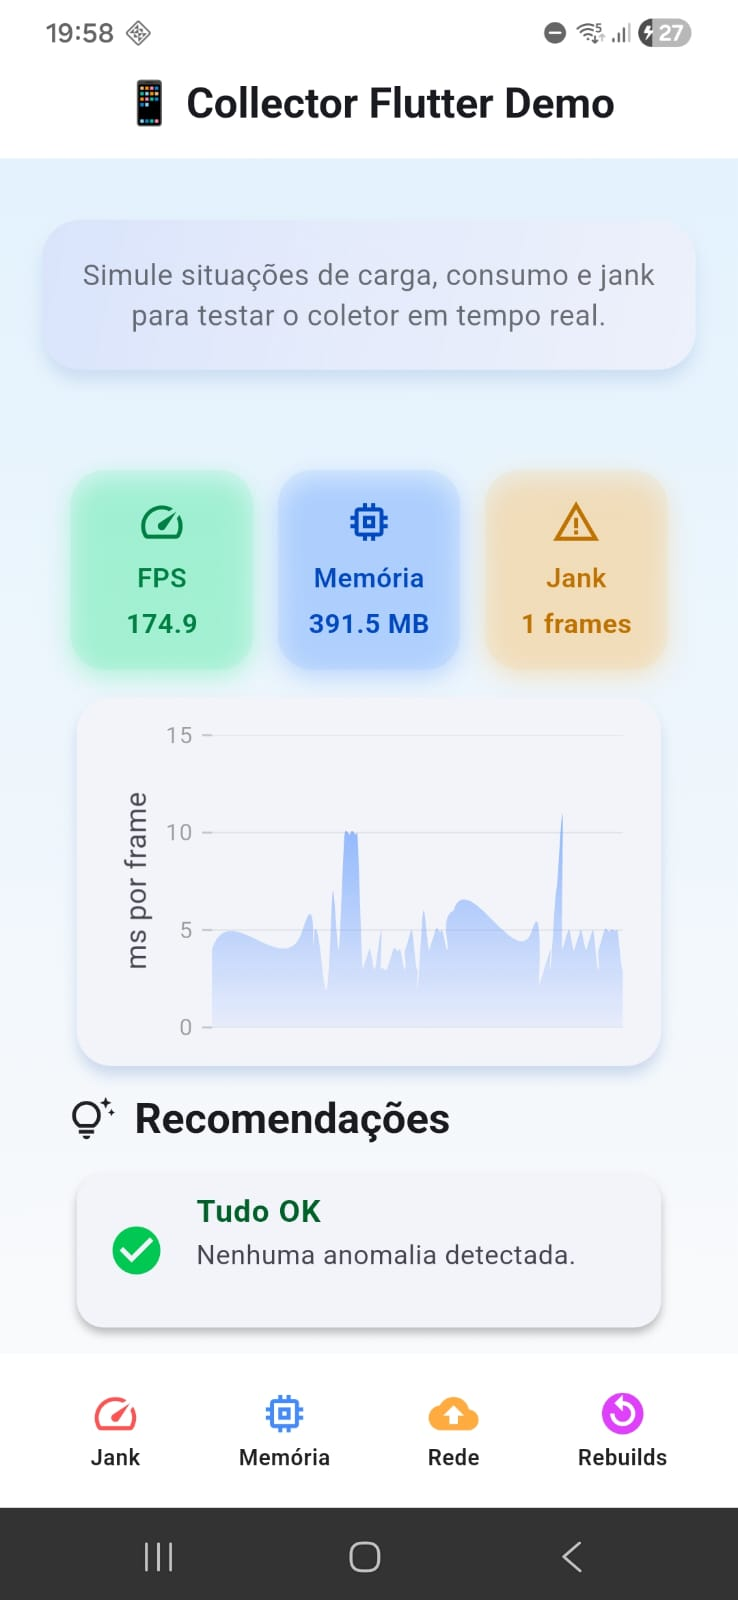
\includegraphics[height=0.8\textwidth]{prototipoquandoestaok.jpeg}
  \caption{Painel do aplicativo em condição de desempenho estável, com indicadores verdes e recomendações informativas.}
  \label{fig:prototype_ok}
\end{figure}

A Figura~\ref{fig:prototype_notok} mostra o comportamento esperado quando há gargalos detectados: os cartões de métricas mudam de cor, o gráfico temporal passa a evidenciar oscilações e as recomendações deixam de ser apenas informativas para orientar possíveis ações de otimização.

\begin{figure}[H]
  \centering
  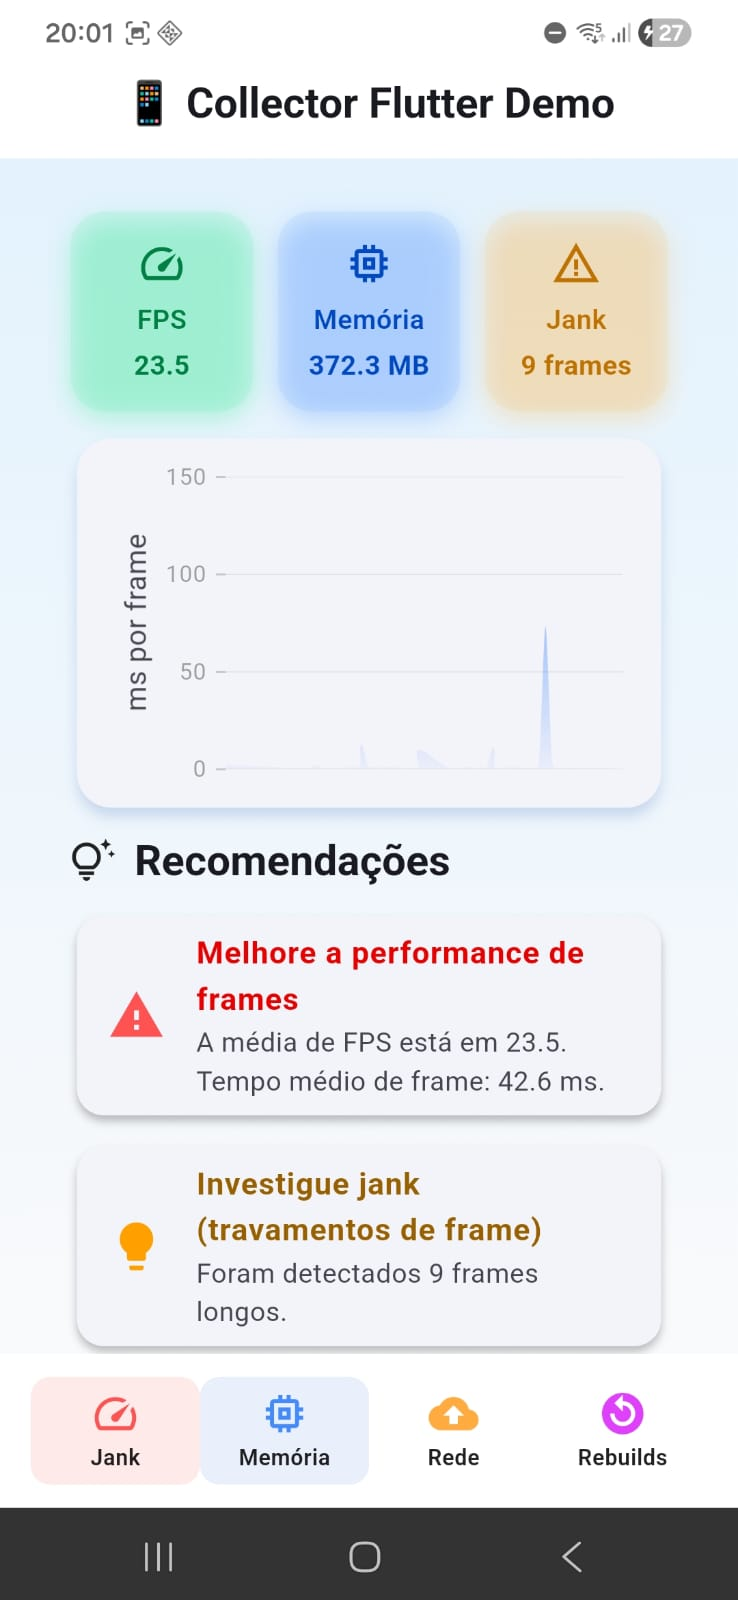
\includegraphics[height=0.8\textwidth]{prototipoquandonaoestaok.jpeg}
  \caption{Painel do aplicativo com anomalias detectadas, como FPS baixo e uso de memória elevado.}
  \label{fig:prototype_notok}
\end{figure}

A Figura~\ref{fig:prototype_icon} identifica o aplicativo de demonstração utilizado nas execuções manuais dos cenários experimentais.

\begin{figure}[H]
  \centering
  
\includegraphics[height=0.3\textwidth]{iconedoappexamplo.jpeg}
  \caption{Ícone do aplicativo de demonstração \texttt{Collector Flutter}.}
  \label{fig:prototype_icon}
\end{figure}


\subsection{Regras de Recomendação}

As recomendações fornecidas pelo módulo \texttt{Recommender} seguem padrões de otimização reconhecidos no ecossistema Flutter e em ferramentas oficiais de diagnóstico~\cite{flutterDevTools2026,android2024}.
Alguns exemplos incluem:

\begin{itemize}
  \item \textbf{Rebuilds frequentes:} “Evite reconstruções excessivas de widgets. Utilize \texttt{const constructors} ou extraia subárvores estáticas.”
  \item \textbf{FPS abaixo de 50:} “Verifique operações pesadas no ciclo de renderização. Considere o uso de \texttt{RepaintBoundary}.”
  \item \textbf{Uso elevado de memória:} “Otimize o descarte de objetos e utilize coleções paginadas.”
  \item \textbf{Chamadas de rede lentas:} “Implemente cache local e controle de tempo de resposta.”
  \item \textbf{Layout sobrecarregado:} “Simplifique hierarquias de widgets e prefira listas com renderização sob demanda, como \texttt{ListView.builder}.”
\end{itemize}

Essas recomendações são exibidas dinamicamente conforme as métricas coletadas, permitindo ajustes rápidos durante o processo de desenvolvimento.

\subsection{Demonstração Prática e Disponibilização do Código-Fonte}

O pacote foi disponibilizado publicamente para garantir transparência e reprodutibilidade dos resultados, conforme recomenda Wohlin \textit{et al.}~\cite{wohlin2012}.

O vídeo de demonstração mostra a execução em tempo real do sistema, com coleta, análise e recomendações heurísticas:

\begin{center}
  \textbf{Acesse o vídeo completo:} \\
  \url{https://drive.google.com/file/d/1KUQ7fFMNRIhe-NSW8loG3wTkQhb_eyOE/view?usp=drive_link}
\end{center}

\noindent
O código-fonte e demais arquivos do projeto estão disponíveis no repositório público:

\begin{center}
  \url{https://github.com/BeatrizVocurcaFrade/collector_flutter}
\end{center}

\noindent
O pacote também foi publicado no repositório oficial do ecossistema Dart/Flutter, permitindo instalação direta e ampliando o acesso da comunidade à ferramenta:

\begin{center}
  \url{https://pub.dev/packages/collector_flutter}
\end{center}

Essa disponibilização em GitHub e pub.dev permite que outros pesquisadores e desenvolvedores avaliem, testem e expandam o sistema, contribuindo para o avanço das pesquisas sobre desempenho e eficiência energética em aplicações Flutter.







% ---------------------------------------------------------------------------------------------------------------------------------------------------------
\section{Critérios de Avaliação}

A validação do pacote \texttt{collector\_flutter} foi conduzida segundo três dimensões efetivamente observadas: \textbf{coerência das métricas coletadas}, \textbf{impacto percebido da coleta} e \textbf{pertinência das recomendações geradas}.
Cada critério foi definido para verificar, de forma funcional, a viabilidade técnica e a aplicabilidade prática do sistema em ambientes reais de desenvolvimento Flutter.



\subsection{Coerência das Métricas Coletadas}

A coerência das métricas foi verificada observando-se se os valores registrados pelo pacote acompanhavam os cenários de carga induzidos no aplicativo de exemplo. Foram analisadas variáveis como tempo médio de renderização de quadros (\textit{frame time}), taxa de quadros por segundo (FPS), consumo de memória, eventos de rede e reconstruções de widgets.

A comparação com ferramentas de referência foi utilizada apenas como apoio qualitativo, sem cálculo formal de erro percentual ou intervalo de confiança. Na versão final documentada, as leituras complementares foram obtidas por \texttt{adb shell dumpsys gfxinfo} e \texttt{adb shell dumpsys meminfo}; Android Profiler e Perfetto permaneceram como referências técnicas do ecossistema, mas não foram empregados como fonte quantitativa de validação.

\subsection{Overhead Introduzido pelo Sistema}

O overhead representa o impacto que o agente de coleta impõe ao desempenho do aplicativo monitorado.
Neste trabalho, esse impacto foi tratado como critério de observação funcional: o coletor deveria permanecer ativo sem impedir a interação com o aplicativo de demonstração nem bloquear a atualização do painel.

Durante os testes, o critério observado foi a manutenção da interação com o aplicativo e da atualização do painel durante a coleta. Não foi realizada mensuração estatística do \textit{overhead}; por isso, os resultados discutem apenas o impacto percebido nas execuções controladas.

\subsection{Eficácia das Recomendações Geradas}

As recomendações heurísticas foram avaliadas verificando-se se o módulo \texttt{Recommender} emitia alertas compatíveis com os gargalos induzidos nos cenários controlados.

Foram analisados sinais como:
\begin{itemize}
  \item \textbf{FPS e \textit{jank}:} recomendações associadas a frames longos e quedas de fluidez;
  \item \textbf{Memória:} alertas relacionados a crescimento sustentado de RSS;
  \item \textbf{Rede:} recomendações diante de volume elevado, falhas ou latência de requisições;
  \item \textbf{Carga combinada:} priorização de recomendações quando múltiplos sintomas ocorrem ao mesmo tempo.
\end{itemize}

\subsection{Clareza da Interface}

A clareza do painel (\texttt{Dashboard}) foi observada por inspeção informal interna durante as execuções manuais, considerando a legibilidade das métricas, a distinção visual dos níveis de severidade e a facilidade de relacionar um alerta ao cenário executado. Essa análise não caracteriza avaliação formal de usabilidade com participantes externos; ela serviu apenas como critério funcional de leitura e interpretação do painel durante os testes.



% ---------------------------------------------------------------------------------------------------------------------------------------------------------



\section{Ferramentas e Ambientes de Desenvolvimento}

O desenvolvimento e a validação do pacote \texttt{collector\_flutter} foram conduzidos em ambiente controlado, com o objetivo de assegurar reprodutibilidade dos resultados e consistência das medições entre diferentes execuções.
As ferramentas selecionadas abrangem IDEs, SDKs e bibliotecas de apoio do ecossistema Flutter, compondo uma infraestrutura moderna, multiplataforma e voltada à análise de desempenho em aplicações Android.

\subsection{Ambientes de Programação e IDEs}

O processo de implementação foi realizado nos seguintes ambientes de desenvolvimento:

\begin{itemize}
  \item \textbf{Visual Studio Code (VS Code):} principal ambiente de escrita e depuração do código Dart e Flutter, configurado com extensões para gerenciamento de pacotes, análise estática e execução de testes unitários.
  \item \textbf{Android Studio:} empregado para execução do aplicativo em dispositivos físicos e emuladores Android, bem como para inspeção complementar de desempenho quando necessário.
\end{itemize}

Ambos os ambientes foram integrados ao controle de versão local via \texttt{Git}, permitindo o gerenciamento seguro e incremental do código-fonte durante o desenvolvimento.

\subsection{SDKs e Dependências Utilizadas}

O ambiente técnico foi configurado com versões estáveis dos SDKs e ferramentas de suporte, garantindo compatibilidade e estabilidade no processo de execução e coleta de métricas:

\begin{itemize}
  \item \textbf{Flutter SDK:} versão \texttt{>=3.22.0} (canal estável), com suporte aos modos \textit{debug}, \textit{profile} e \textit{release}.
  \item \textbf{Dart SDK:} versão correspondente ao Flutter 3.22, utilizada para o desenvolvimento dos módulos de coleta e análise de dados.
  \item \textbf{Android SDK:} configurado com as APIs 33 e 34, compatíveis com Android 12 e 13.
  \item \textbf{Gradle:} atualizado para suportar as dependências do projeto e a integração com o Android Studio.
\end{itemize}

Essa configuração assegura a execução consistente do pacote em diferentes dispositivos Android, com coleta precisa de métricas e comportamento previsível.

\subsection{Ambientes de Teste e Dispositivos}

Os testes experimentais foram realizados exclusivamente em ambiente Android, com dispositivos físicos e emulados representando diferentes capacidades de processamento e arquiteturas.

\begin{itemize}
  \item \textbf{Dispositivos físicos:}
    \begin{itemize}
      \item Samsung Galaxy A52, Android 13;
      \item Motorola G73, Android 12.
    \end{itemize}
  \item \textbf{Emuladores Android:}
    \begin{itemize}
      \item Pixel 6 (x86\_64), Android 14, configurado via Android Studio.
    \end{itemize}
\end{itemize}

Todos os testes foram conduzidos em modo \textit{profile}, permitindo medições precisas de tempo de renderização, FPS e consumo de recursos em condições controladas.

\subsection{Ferramentas de Referência e Validação}

A validação dos resultados obtidos pelo pacote foi realizada com apoio de ferramentas oficiais do ecossistema Android, utilizadas como referência qualitativa para as métricas coletadas:

\begin{itemize}
  \item \textbf{ADB (\textit{Android Debug Bridge}):} empregado para a coleta de informações complementares sobre memória do processo e desempenho de quadros por meio dos comandos \texttt{dumpsys meminfo} e \texttt{dumpsys gfxinfo}.
  \item \textbf{Android Profiler e Perfetto:} utilizados como referências conceituais e ferramentas oficiais de diagnóstico do ecossistema Android, mas sem geração de série comparativa quantitativa neste trabalho.
\end{itemize}

Essas ferramentas apoiaram a interpretação dos resultados, permitindo verificar se os sinais exibidos pelo painel acompanhavam o comportamento esperado dos cenários. A comparação permaneceu qualitativa e não caracteriza medição estatística de precisão.

\subsection{Frameworks e Bibliotecas de Apoio}

Durante o desenvolvimento, foram utilizadas bibliotecas consolidadas do ecossistema Flutter/Dart, responsáveis por facilitar a instrumentação, visualização de dados e controle de estado da aplicação:

\begin{itemize}
  \item \textbf{\texttt{flutter\_bloc}:} gerenciamento reativo de estado, responsável pela comunicação entre coleta, análise e exibição das métricas.
  \item \textbf{\texttt{fl\_chart}:} biblioteca de visualização gráfica utilizada na renderização dos gráficos em tempo real no painel interno (\textit{Dashboard}).
  \item \textbf{\texttt{http}:} responsável pela instrumentação e monitoramento das requisições de rede durante a execução do aplicativo.
  \item \textbf{\texttt{connectivity\_plus}:} monitora eventos de conectividade e simula condições de rede variável.
  \item \textbf{\texttt{logger}:} realiza o registro estruturado de eventos e mensagens internas do sistema, facilitando a depuração.
  \item \textbf{\texttt{vm\_service}:} fornece acesso às APIs internas da máquina virtual Dart, permitindo capturar dados de alocação e uso de memória.
\end{itemize}

Essas dependências foram selecionadas por sua estabilidade, compatibilidade com o ambiente de testes Android e suporte nativo ao desenvolvimento em Dart puro, sem componentes externos.

\subsection{Ambientes de Testes Automatizados}

A confiabilidade do sistema foi verificada por meio de testes unitários e execuções manuais controladas. Essa abordagem garantiu a validação tanto da lógica interna quanto do comportamento visual e interativo do painel.

\begin{itemize}
  \item \textbf{Testes unitários:} implementados com o pacote \texttt{flutter\_test}, abrangendo módulos de coleta e análise (\texttt{Collector}, \texttt{Analyzer} e \texttt{Recommender}).
  Esses testes asseguram que cada componente produza resultados consistentes e corretos em diferentes condições de entrada.
  \item \textbf{Testes manuais:} realizados diretamente em dispositivos físicos e emuladores, com execução de cenários controlados (rebuilds em massa, requisições de rede intensas, simulação de carga de CPU) para observar o comportamento do sistema em tempo real.
\end{itemize}

Essa combinação de testes unitários e manuais possibilitou uma avaliação funcional da coerência das métricas e da estabilidade geral do pacote durante o uso prático.

\vspace{0.5em}

A infraestrutura descrita nesta seção assegura que o pacote \texttt{collector\_flutter} seja executado de forma estável e reproduzível, permitindo uma análise detalhada do desempenho e da eficiência de aplicações Flutter em ambiente Android.

% !TEX root = ../Monografia.tex
% ---------------------------------------------------------------------------------------------------------------------------------------------------------
\section{Procedimentos de Teste e Coleta de Dados}
% ---------------------------------------------------------------------------------------------------------------------------------------------------------

Esta seção descreve os procedimentos utilizados para validar funcionalmente o protótipo \texttt{collector\_flutter}. O objetivo principal dos testes foi observar três aspectos fundamentais do sistema: (i) a coerência das métricas coletadas, (ii) o impacto percebido da coleta durante a execução e (iii) a pertinência das recomendações heurísticas geradas pelo sistema.

Para garantir validade científica e reprodutibilidade, os testes foram conduzidos em ambiente controlado, seguindo protocolos experimentais inspirados nas diretrizes de experimentação em engenharia de software propostas por Wohlin \textit{et al.}~\cite{wohlin2012}.

\subsection{Protocolo de Execução dos Testes}

Os experimentos foram executados em modo \textit{profile} do Flutter, pois esse modo permite medições mais próximas do comportamento real da aplicação, eliminando interferências associadas ao modo \textit{debug}. Antes de cada execução experimental, o dispositivo foi reiniciado e o aplicativo executado em estado limpo, garantindo consistência entre as medições.

O protocolo de execução foi composto pelas seguintes etapas:

\begin{enumerate}

\item \textbf{Preparação do ambiente}: reinicialização do dispositivo e encerramento de processos em segundo plano, assegurando estabilidade do ambiente de execução.

\item \textbf{Inicialização do coletor}: ativação do módulo \texttt{ResourceCollector} por meio do método \texttt{start()}, responsável por iniciar a captura das métricas de desempenho.

\item \textbf{Execução do cenário experimental}: cada cenário foi acionado no aplicativo de exemplo por tempo suficiente para observar a reação do coletor e do painel visual.

\item \textbf{Registro das métricas}: durante a execução do cenário, o coletor registrou continuamente métricas de desempenho relacionadas à renderização, uso de memória, chamadas de rede e reconstruções de widgets.

\item \textbf{Encerramento da coleta}: ao término do experimento, o método \texttt{stop()} foi acionado e os dados coletados foram exportados para arquivos estruturados no formato JSON.

\end{enumerate}

Os cenários foram executados manualmente em condições controladas, com o objetivo de verificar a operacionalidade do sistema e identificar inconsistências nas heurísticas. Os resultados apresentados neste trabalho são de natureza qualitativa.

\subsection{Definição dos Cenários Experimentais}

Quatro cenários experimentais foram definidos com o objetivo de simular diferentes tipos de carga comuns em aplicações móveis. Cada cenário foi projetado para provocar um tipo específico de comportamento de desempenho.

\begin{itemize}

\item \textbf{Cenário 1 – Reconstruções intensivas de interface}

Neste cenário, um conjunto de widgets foi reconstruído repetidamente em alta frequência, simulando aplicações com atualização constante de interface. Esse cenário foi utilizado para avaliar o impacto das reconstruções de widgets sobre o tempo de renderização e o FPS.

\item \textbf{Cenário 2 – Chamadas de rede simultâneas}

Foram disparadas múltiplas requisições HTTP paralelas, utilizando o método \texttt{recordNetwork()}, com o objetivo de observar o comportamento do sistema sob carga de rede e verificar a capacidade do coletor de registrar eventos relacionados a comunicação externa.

\item \textbf{Cenário 3 – Alocação intensiva de memória}

Objetos de grande volume foram criados e descartados continuamente durante a execução do teste. Esse cenário permitiu analisar padrões de uso de memória e observar eventos de coleta de lixo (\textit{garbage collection}).

\item \textbf{Cenário 4 – Carga combinada}

Neste cenário, os três tipos de carga anteriores foram executados simultaneamente, simulando um comportamento mais próximo de aplicações reais, nas quais operações de interface, rede e memória ocorrem de forma concorrente.

\end{itemize}

Esses cenários permitiram avaliar o comportamento do sistema em diferentes condições de uso, identificando possíveis limitações e avaliando a robustez da ferramenta.

\subsection{Coleta de Métricas}

As métricas foram coletadas automaticamente pelo módulo \texttt{Collector}, implementado inteiramente em Dart. A captura dos dados foi realizada em tempo real utilizando \texttt{Streams} internas do Flutter.

As métricas analisadas foram:

\begin{itemize}

\item \textbf{FPS (Frames por Segundo)}: indicador da fluidez da renderização da interface;

\item \textbf{Tempo médio de renderização de quadro}: calculado a partir dos eventos de \texttt{FrameTiming};

\item \textbf{Número de reconstruções de widgets}: contabilizado por meio do componente \texttt{RebuildObserver};

\item \textbf{Uso de memória}: obtido via API \texttt{vmService.getAllocationProfile()};

\item \textbf{Número de chamadas de rede}: monitorado por meio da instrumentação do método \texttt{recordNetwork()}.

\end{itemize}

Os dados coletados foram serializados em formato JSON estruturado, permitindo inspeção posterior e reprodutibilidade dos registros observados.

\subsection{Métodos de Comparação}

Para apoiar a verificação das medições obtidas pelo protótipo, os resultados foram confrontados qualitativamente com ferramentas oficiais de análise de desempenho do ecossistema Android.

As ferramentas utilizadas como referência foram:

\begin{itemize}

\item \textbf{Android Profiler}, utilizado para medir consumo de CPU, memória e FPS;

\item \textbf{ADB (\texttt{adb shell dumpsys gfxinfo})}, utilizado para obter métricas detalhadas de renderização de quadros.

\end{itemize}

A comparação quantitativa por erro percentual não foi executada nesta versão, mas a expressão abaixo documenta o cálculo previsto para estudos futuros:

\[
Erro (\%) = \frac{|M_{ref} - M_{proto}|}{M_{ref}} \times 100
\]

onde \(M_{ref}\) representa o valor obtido pela ferramenta de referência e \(M_{proto}\) representa o valor registrado pelo protótipo.

\subsection{Análise dos Resultados}

Os dados coletados foram analisados de forma qualitativa, considerando a coerência entre o cenário acionado, as métricas exibidas no painel e as recomendações emitidas pelo módulo \texttt{Recommender}.

Além disso, o \textit{overhead} foi tratado como critério metodológico para avaliações futuras, comparando o tempo médio de renderização de quadros com o sistema ativado e desativado.

O cálculo previsto utiliza a seguinte expressão:

\[
Overhead (\%) = \frac{T_{com} - T_{sem}}{T_{sem}} \times 100
\]

onde \(T_{com}\) representa o tempo médio de execução com o coletor ativado e \(T_{sem}\) corresponde ao tempo de execução sem monitoramento.

\subsection{Controle Experimental e Reprodutibilidade}

Para garantir a validade experimental dos resultados, foram adotadas medidas de controle que minimizam interferências externas durante os testes:

\begin{itemize}

\item execução em modo \textit{profile};

\item utilização das mesmas versões do Flutter SDK e dependências em todas as execuções;

\item execução dos testes em ambiente com temperatura e carga de bateria estáveis;

\item repetição manual dos cenários quando necessário para confirmar o comportamento observado;

\item padronização do formato de saída das métricas em arquivos JSON.

\end{itemize}

Essas práticas auxiliam a reprodução dos cenários por outros pesquisadores, reforçando a transparência da avaliação funcional do protótipo \texttt{collector\_flutter}.
\begin{table}[H]
\centering
\caption{Resumo dos cenários experimentais utilizados nos testes.}
\begin{tabular}{|c|p{4cm}|p{6cm}|}
\hline
\textbf{Cenário} & \textbf{Tipo de Carga} & \textbf{Objetivo} \\
\hline
1 & Reconstruções de interface & Avaliar impacto de rebuilds frequentes na renderização \\
\hline
2 & Chamadas de rede simultâneas & Observar comportamento sob múltiplas requisições HTTP \\
\hline
3 & Alocação intensiva de memória & Identificar padrões de consumo e eventos de garbage collection \\
\hline
4 & Carga combinada & Simular comportamento próximo de aplicações reais \\
\hline
\end{tabular}
\end{table}

% !TEX root = ../Monografia.tex
% ---------------------------------------------------------
% BIBLIOGRAFIA
% ---------------------------------------------------------
\begin{thebibliography}{99}

% ---------------------------------------------------------
% TRABALHOS ACADÊMICOS RELACIONADOS
% ---------------------------------------------------------

\bibitem{pathak2012energy}
PATHAK, A.; HU, Y. C.; ZHANG, M.
\newblock \textit{Fine-grained Power Modeling for Smartphones Using System Call Tracing}.
\newblock In: \emph{Proceedings of the European Conference on Computer Systems}.
\newblock ACM, 2012.

\bibitem{liu2019profiling}
LIU, Y.; ZHOU, X.; ZHANG, H.
\newblock \textit{Profiling and Diagnosing Performance Issues in Mobile Applications}.
\newblock \emph{IEEE Software}, v. 36, n. 5, p. 80–87, 2019.

\bibitem{he2019crossplatform}
HE, J.; LI, S.; WANG, Y.
\newblock \textit{Performance Comparison of Cross-Platform Mobile Development Frameworks}.
\newblock \emph{Journal of Systems and Software}, v. 152, p. 1–16, 2019.

\bibitem{banerjee2020automated}
BANERJEE, S.; ROY, S.; DUTTA, K.
\newblock \textit{Automated Runtime Monitoring for Mobile Applications}.
\newblock \emph{ACM Transactions on Software Engineering and Methodology}, v. 29, n. 4, 2020.

\bibitem{hao2013estimating}
HAO, S.; LI, D.; HALFOND, W.
\newblock \textit{Estimating Mobile Application Energy Consumption Using Program Analysis}.
\newblock In: \emph{Proceedings of the International Conference on Software Engineering (ICSE)}.
\newblock IEEE, 2013.

\bibitem{li2014empirical}
LI, D.; HALFOND, W.
\newblock \textit{An Empirical Study of Energy Consumption of Android Applications}.
\newblock In: \emph{International Conference on Software Maintenance and Evolution}.
\newblock IEEE, 2014.

% ---------------------------------------------------------
% TRABALHOS ACADÊMICOS (TCC / DISSERTAÇÕES)
% ---------------------------------------------------------

\bibitem{silva2022mobile}
SILVA, R. A.
\newblock \textit{Análise de Consumo Energético em Aplicações Móveis Android}.
\newblock Dissertação (Mestrado em Ciência da Computação) – Universidade Federal de Pernambuco, 2022.

\bibitem{santos2023flutter}
SANTOS, L. F.
\newblock \textit{Avaliação de Desempenho em Aplicações Flutter: Um Estudo Experimental}.
\newblock Trabalho de Conclusão de Curso – Universidade de São Paulo, 2023.

\bibitem{rodrigues2021mobile}
RODRIGUES, M. P.
\newblock \textit{Ferramentas de Monitoramento de Desempenho em Aplicações Móveis}.
\newblock Trabalho de Conclusão de Curso – Universidade Federal de Minas Gerais, 2021.

% ---------------------------------------------------------
% DOCUMENTAÇÃO DE FERRAMENTAS
% ---------------------------------------------------------

\bibitem{android2024}
ANDROID DEVELOPERS.
\newblock \textbf{Android Profiler}.
\newblock Disponível em: \url{https://developer.android.com/studio/profile}.
\newblock Acesso em: 05 out. 2025.

\bibitem{aosp2024}
ANDROID OPEN SOURCE PROJECT.
\newblock \textbf{Perfetto Tracing}.
\newblock Disponível em: \url{https://perfetto.dev}.
\newblock Acesso em: 05 out. 2025.

\bibitem{apple2024}
APPLE.
\newblock \textbf{Xcode Instruments}.
\newblock Disponível em: \url{https://developer.apple.com/xcode/instruments/}.
\newblock Acesso em: 05 out. 2025.

\bibitem{meta2024}
META.
\newblock \textbf{Flipper – React Native Debugging Tool}.
\newblock Disponível em: \url{https://fbflipper.com}.
\newblock Acesso em: 05 out. 2025.

\bibitem{google2024devtools}
GOOGLE.
\newblock \textbf{Flutter DevTools}.
\newblock Disponível em: \url{https://docs.flutter.dev/development/tools/devtools/overview}.
\newblock Acesso em: 05 out. 2025.

\bibitem{google2023flutter}
GOOGLE.
\newblock \textbf{Flutter: Build Apps for Any Screen}.
\newblock Disponível em: \url{https://flutter.dev}.
\newblock Acesso em: 22 ago. 2025.

\bibitem{meyer2022performance}
MEYER, J.; KRAUSE, A.
\newblock \textit{Performance Evaluation of Flutter vs React Native in Production Environments}.
\newblock \emph{International Journal of Mobile Computing and Multimedia Communications}, v. 8, n. 2, p. 112--125, 2022.

\bibitem{dart2023}
DART TEAM.
\newblock \textbf{Dart: A Client-Optimized Language for Fast Apps on Any Platform}.
\newblock Disponível em: \url{https://dart.dev}.
\newblock Acesso em: 22 ago. 2025.

% ---------------------------------------------------------
% ARTIGOS SOBRE ENERGIA E DESEMPENHO
% ---------------------------------------------------------

\bibitem{cheng2020energy}
CHENG, L.; WANG, X.
\newblock \textit{Energy Consumption Analysis in Mobile Applications: A Framework-based Approach}.
\newblock \emph{Journal of Software Engineering}, 15(4), 45–59, 2020.

\bibitem{zhang2021energy}
ZHANG, Y.; LIU, J.; CHEN, F.
\newblock \textit{Evaluating Energy Efficiency of Flutter and React Native Applications}.
\newblock In: \emph{Proceedings of the International Conference on Mobile Systems}.
\newblock ACM, 2021.

\bibitem{johnson2020monitoring}
JOHNSON, R.
\newblock \textit{Monitoring System Calls and Frame Rendering Events for Energy Optimization}.
\newblock \emph{Software: Practice and Experience}, 50(9), 1652–1668, 2020.

\bibitem{kumar2019optimization}
KUMAR, P.; GUPTA, R.
\newblock \textit{Optimizing Resource Consumption in Mobile Apps: Techniques and Tools}.
\newblock \emph{International Journal of Software Engineering}, 12(4), 234–250, 2019.

% ---------------------------------------------------------
% SUSTENTABILIDADE
% ---------------------------------------------------------

\bibitem{google2024sustainability}
GOOGLE SUSTAINABILITY.
\newblock \textbf{Reducing Energy Consumption in Software}.
\newblock Disponível em: \url{https://sustainability.google}.
\newblock Acesso em: 05 out. 2025.

\bibitem{ieee2023sustainability}
IEEE.
\newblock \textbf{Sustainability in Software Engineering}.
\newblock Disponível em: \url{https://www.ieee.org/sustainability}.
\newblock Acesso em: 05 out. 2025.

\bibitem{unep2023}
UNITED NATIONS ENVIRONMENT PROGRAMME (UNEP).
\newblock \textbf{Digital Sustainability Initiatives}.
\newblock Disponível em: \url{https://www.unep.org/resources}.
\newblock Acesso em: 05 out. 2025.

% ---------------------------------------------------------
% METODOLOGIA CIENTÍFICA
% ---------------------------------------------------------

\bibitem{gil2017}
GIL, A. C.
\newblock \textbf{Métodos e Técnicas de Pesquisa Social}.
\newblock 7. ed. São Paulo: Atlas, 2017.

\bibitem{lakatos2021}
LAKATOS, E. M.; MARCONI, M. A.
\newblock \textbf{Fundamentos de Metodologia Científica}.
\newblock 9. ed. São Paulo: Atlas, 2021.

\bibitem{yin2015}
YIN, R. K.
\newblock \textbf{Estudo de Caso: Planejamento e Métodos}.
\newblock 5. ed. Porto Alegre: Bookman, 2015.

\bibitem{wohlin2012}
WOHLIN, C. et al.
\newblock \textbf{Experimentation in Software Engineering}.
\newblock Springer, 2012.

% ---------------------------------------------------------
% ENGENHARIA DE SOFTWARE
% ---------------------------------------------------------

\bibitem{pressman2020engenharia}
PRESSMAN, R. S.; MAXIM, B. R.
\newblock \textbf{Engenharia de Software: Uma Abordagem Profissional}.
\newblock 9. ed. Porto Alegre: AMGH, 2020.

\bibitem{kitchenham2007guidelines}
KITCHENHAM, B.; CHARTERS, S.
\newblock \textbf{Guidelines for Performing Systematic Literature Reviews in Software Engineering}.
\newblock EBSE Technical Report, Keele University, 2007.

\bibitem{sommerville2019software}
SOMMERVILLE, I.
\newblock \textbf{Engenharia de Software}.
\newblock 10. ed. São Paulo: Pearson, 2019.

\bibitem{martin2018clean}
MARTIN, R. C.
\newblock \textbf{Clean Architecture: A Craftsman’s Guide to Software Structure and Design}.
\newblock Prentice Hall, 2018.

\bibitem{evans2004domain}
EVANS, E.
\newblock \textbf{Domain-Driven Design: Tackling Complexity in the Heart of Software}.
\newblock Addison-Wesley, 2004.

% ---------------------------------------------------------
% REFERÊNCIAS ADICIONADAS NA REVISÃO (verificar antes da defesa)
% Fontes identificadas em IEEE Xplore, ACM DL, arXiv e Springer.
% ---------------------------------------------------------

\bibitem{ravindranath2012appinsight}
RAVINDRANATH, L.; PADHYE, J.; AGARWAL, S.; MAHAJAN, R.; OBERMILLER, I.; SHAYANDEH, S.
\newblock \textit{AppInsight: Mobile App Performance Monitoring in the Wild}.
\newblock In: \emph{Proceedings of the 10th USENIX Symposium on Operating Systems Design and Implementation (OSDI 12)}.
\newblock USENIX Association, 2012. p. 107--120.

\bibitem{verma2023largescale}
VERMA, A.; TRIVEDI, A.; PANDEY, H. M.
\newblock \textit{A large-scale empirical study on mobile performance: energy, run-time and memory}.
\newblock \emph{Empirical Software Engineering}, v. 28, art. 161, 2023.
\newblock DOI: 10.1007/s10664-023-10391-y.

\bibitem{horn2023nativeweb}
HORN, R. et al.
\newblock \textit{Native vs Web Apps: Comparing the Energy Consumption and Performance of Android Apps and their Web Counterparts}.
\newblock In: \emph{Proceedings of the 10th International Conference on Mobile Software Engineering and Systems (MOBILESoft)}.
\newblock ACM, 2023.

\bibitem{dornauer2023energysaving}
DORNAUER, B.; FELDERER, M.
\newblock \textit{Energy-Saving Strategies for Mobile Web Apps and their Measurement: Results from a Decade of Research}.
\newblock In: \emph{Proceedings of the 10th International Conference on Mobile Software Engineering and Systems (MOBILESoft)}.
\newblock ACM, 2023.

\bibitem{sun2023energyinefficiency}
SUN, Y. et al.
\newblock \textit{Energy inefficiency diagnosis for Android applications: a literature review}.
\newblock \emph{Frontiers of Computer Science}, v. 17, n. 1, art. 171201, 2023.
\newblock DOI: 10.1007/s11704-021-0532-4.

\bibitem{toni2023apienergy}
TONI, C. et al.
\newblock \textit{Energy-Consumption Estimation of API-usage in Smartphone Apps via Static Analysis}.
\newblock In: \emph{Proceedings of the 20th International Conference on Mining Software Repositories (MSR)}.
\newblock IEEE, 2023.
\newblock DOI: 10.1109/MSR59073.2023.00057.

\end{thebibliography}

\end{document}
